%!TEX ROOT = thesis.tex
\chapter{Methodology}

\hspace{12.7mm}\hl{This chapter presents the research methodology that was designed to address the research gaps identified in the literature. Each gap is met by a specific component of the methodology. The lack of external validation and calibration is addressed by testing the models on external data and assessing their calibration and
clinical utility. The class overlap is handled by guiding the feature selection and the data resampling with class overlap measures. The limited use of actionable explanations is addressed by counterfactual explanations. The chapter starts with the theoretical framework of the study, followed by an overview of the methodology framework and a detailed description of its stages.}

\section{Theoretical Framework}
\hl{The theoretical framework of this research is based on the understanding of cognitive impairment as the outcome of neuropathological changes, such as the accumulation of amyloid-beta and tau proteins or vascular damage. These changes progress gradually and begin years before any clinical diagnosis is reached} \cite{Beason-Held2013Changes}. \hl{The condition is not a single disease but a group of subtypes with different causes, such as Alzheimer's disease, which makes both diagnosis and prediction more difficult} \cite{Scheltens2021Alzheimer}. \hl{In clinical practice, the cognitive status of a patient is determined by following recognized diagnostic frameworks. For instance, the National Institute on Aging and the Alzheimer's Association (NIA-AA)} \cite{Besser2018Version} \hl{define dementia and its stages from the patient history, cognitive testing, and functional assessment, while the Clinical Dementia Rating is commonly used to grade disease severity} \cite{Morris1993Clinical}.

\hl{Accessible data can be used to approximate the clinical diagnosis of cognitive impairment. A large part of dementia risk is attributed to modifiable risk factors, such as hypertension, diabetes, depression, and physical inactivity, which are recorded in routine health history and lifestyle information} \cite{Livingston2020Dementia}. \hl{In addition, the disease produces gradual changes in daily functioning and behavior before a formal diagnosis is made, and these changes can be captured by simple functional and behavioral assessments} \cite{Beason-Held2013Changes}. \hl{Therefore, accessible variables can serve as early signs of the presence of cognitive impairment, and such a relationship can be analyzed to predict the current and future cognitive status. However, this relationship is complex because the accessible variables have a weak effect and interact in non-linear ways that might differ between dementia subtypes. Such a complex relationship is difficult to capture using simple rules.} 

\hl{Machine learning is suitable for this setting because it learns the relationship directly from labeled data without being explicitly programmed. This is supported by statistical learning theory, which shows that a learning algorithm can learn the relationship between the features and the outcome from a set of examples and then apply it to new patients} \cite{Hastie2009Elements}. \hl{Since models statistically learn to approximate the clinical diagnosis from the data, they should be used to support clinical decision-making rather than replace it. For the models to be clinically useful, they should be cost-effective, accurate, generalizable, and interpretable (a formal definition of a cost-effective model is provided in the Glossary, } Table~\ref{table:glossary}). \hl{The cost-effectiveness of the models can be achieved by using accessible data and optimizing the modeling process to reduce computational cost. With regard to accuracy, the gradual nature of cognitive decline creates overlapping boundaries between adjacent stages, which makes it challenging for cost-effective models to accurately distinguish between them. Applying appropriate data preprocessing techniques can increase the performance of the models by minimizing class overlap. As for interpretability, it is crucial to provide transparent and personalized explanations of the model's predictions to build clinical trust and to generate actionable insights for the management of cognitive risk} \cite{Martin2023Interpretable}. \hl{Guided by this theoretical framework, the following section presents the research methodology framework adopted to develop the proposed models.}

\section{Overview of Research Methodology Framework}
This research is based on a methodological framework that follows an experimental data-driven approach to assess the feasibility and effectiveness of developing machine learning models for the early prediction of cognitive impairment (\acrshort{CI}). Refer to Figure~\ref{fig:research-method-diagram} for the research methodology framework diagram. The entire research methodology was structured to fulfill the research objectives and address the identified gaps in the literature. The research methodology consists of a multiple-stage process that includes data acquisition, data preprocessing, and model fine-tuning, validation, and explanation. During the data preprocessing phase, dataset segmentation for hierarchical classification tasks is performed. Subsequently, the National Alzheimer's Coordinating Center Uniform Data Set (\acrshort{NACC} \acrshort{UDS}) is split into training and cross-center testing datasets based on research centers. Furthermore, preprocessing steps are performed to the training dataset, and the fitted parameters from the preprocessing steps are applied to the testing dataset to ensure a robust evaluation. 

\begin{figure}[ht]
    \centering
    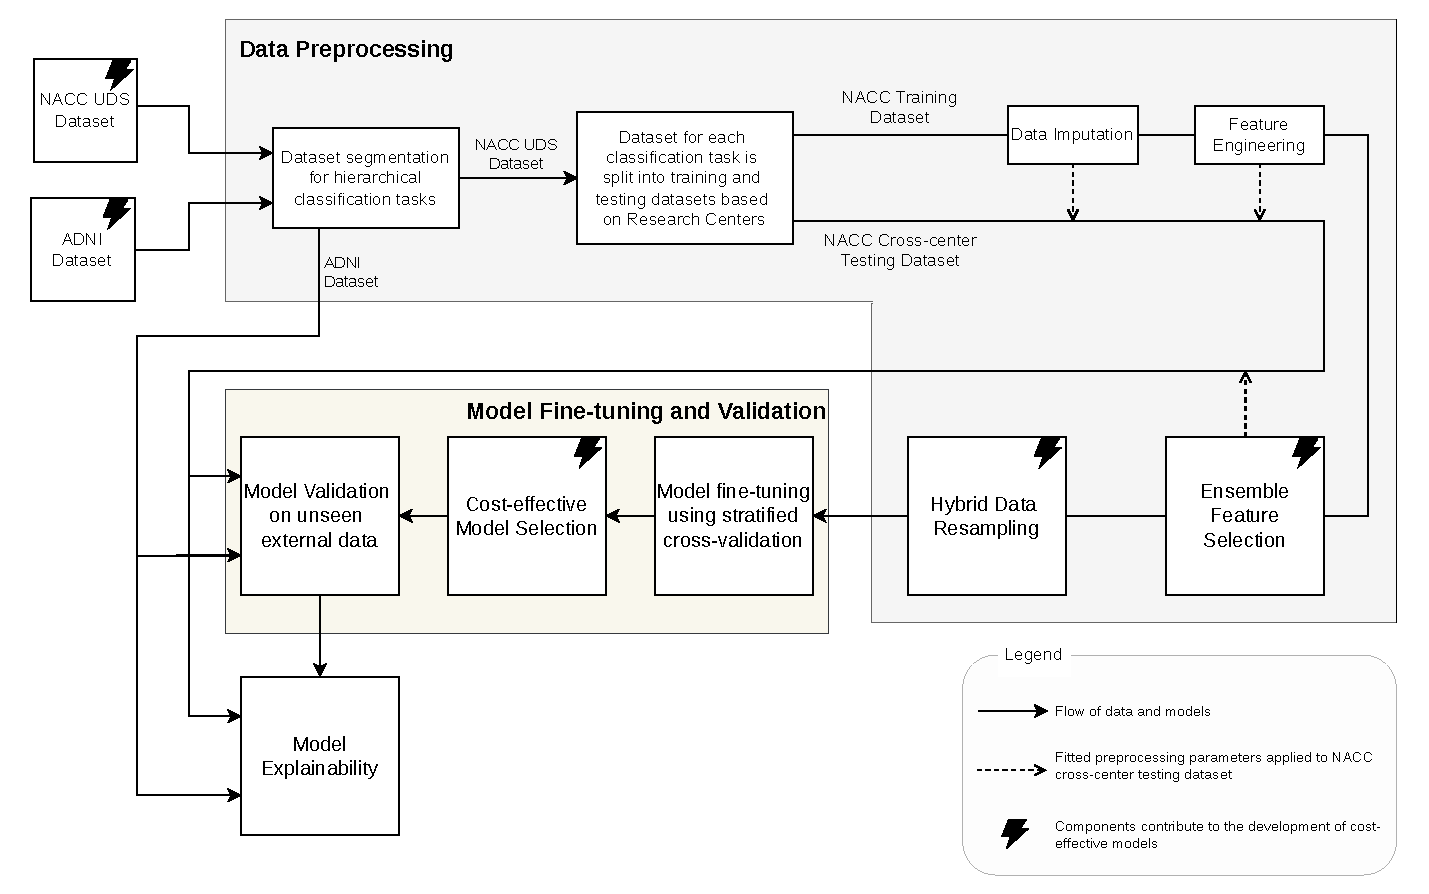
\includegraphics[width=\textwidth]{figures/research-framework.pdf}
    \caption{The research methodology framework diagram}
    \label{fig:research-method-diagram}
\end{figure}

Multiple machine learning algorithms were evaluated for predictive performance, computational efficiency, and interpretability. These models were trained in easily accessible features, such as demographics, health history, and basic assessment of behavior and cognitive functionality. The selected models were tested using external test data, specifically the Alzheimer’s Disease Neuroimaging Initiative (\acrshort{ADNI}) dataset, to assess their generalizability. A comprehensive assessment of the performance and calibration of the selected models were conducted. The methodology also incorporates Explainable Artificial Intelligence (\acrshort{XAI}) techniques to provide transparency in decision-making.

\hl{The development of cost-effective models is achieved through four main components in the proposed research methodology. The first component is the use of accessible data from both the NACC UDS and ADNI datasets. The second and third components are the ensemble feature selection and the hybrid data resampling, both of which reduce the feature subset and computational cost. The fourth component is the cost-effective model selection, which uses a novel algorithm to select faster and more efficient models while maintaining an acceptable performance.}

The research methodology was designed to handle the classification challenges of using accessible data, such as class imbalance and class overlap. It also promotes the development of cost-effective and generalizable models through optimized fine tuning and robust external validation. This research approach ensures clinical relevance and feasibility in real-world healthcare settings. In addition, the study methodology and results were reported according to the TRIPOD+AI guidelines \cite{Collins2024TRIPOD+AI}. The methods of this research are discussed in more detail in the sections of this chapter.

\section{Dataset Description}
The data in this study were obtained from two different datasets commonly used in the literature to implement robust model development and validation methods. The following subsections introduce the utilized datasets.

\subsection{National Alzheimer's Coordinating Center Uniform Data Set}
The main dataset used in this study is the Uniform Data Set (\acrshort{UDS}) provided by the National Alzheimer's Coordinating Center (\acrshort{NACC}) \cite{Beekly2007National}. The dataset is based on the UDS data freeze in March 2025. The dataset was collected through a longitudinal clinical evaluation of 44,713 subjects from 43 Alzheimer's disease research centers (\acrshort{ADRCs}) across the United States, starting from September 2005. Subjects have participated in annual visits by completing 16 forms related to multiple topics, including subject demographics, health history, neurological assessments, and diagnosis. Initial and follow-up visits have been made in person or through telephone calls. The total number of visits made by each subject ranged from one visit to 20 visits (mean = 3.85 and standard deviation = 3.15). The UDS forms have evolved into multiple versions since their inception in 2005. The utilization of the 2011 NIA-AA criteria for Alzheimer’s disease was among the updates during the major upgrade from version 2 to version 3 in 2015 \cite{Besser2018Version}. Some variables in UDS are only collected in some versions or were collected with different methods across versions. \hl{The complete list of the initially selected accessible variables extracted from the NACC UDS is provided in} Table~\ref{table:initial-uds-variables} in the appendix.

The NACC UDS is distinguished by its standardized longitudinal data collection, which captures information over multiple visits from large and diverse populations across multiple ADRCs in the United States. It is publicly available for research purposes and has been used in recent studies focused on developing predictive machine learning models \cite{abbas2024Explainable, Pang2023Predicting, Ren2023Improving}. It provides a wide range of easily accessible data, including demographic, health history, lifestyle factors, and cognitive assessments collected during routine medical examinations. This variety allows for comprehensive analysis and makes the dataset practical for clinical applications. Additionally, the NACC UDS encompasses a broad spectrum of cognitive status and various types of dementia, with diagnoses being recorded over time at multiple visits. This enables the development of models capable of predicting the risk of different types of dementia in the early stages. Moreover, data collected from ADRCs in different geographic regions with unique demographic, socioeconomic, and healthcare characteristics offers an opportunity to test the model’s ability to generalize across diverse clinical environments. These advantages collectively make the NACC UDS more practical for this study than other commonly used datasets. This decision supports the objectives of this study to develop generalizable and accessible models for the early prediction and intervention of cognitive impairment in clinical practice.

\hl{In addition to these advantages, the demographic composition of the NACC UDS cohort was examined. The subjects are mostly older adults, typically aged between about 60 and 80 years. The majority of subjects are female, and the level of education is relatively high, with a mean of around 15 years. The data are restricted to the United States, and some racial and ethnic groups are likely to be underrepresented. This pattern is commonly noted in dementia cohorts} \cite{Lennon2021Black, Nianogo2022Risk}. \hl{The NACC UDS is also a convenience sample of subjects attending Alzheimer's disease research centers, which explains the high prevalence of cognitive impairment in the data. This demographic skew has a direct impact on the generalizability of the models, since a model that learns from such data may not behave equally well when it meets populations of different demographic and socioeconomic backgrounds.}

\subsection{Alzheimer's Disease Neuroimaging Initiative Dataset}
The Alzheimer's Disease Neuroimaging Initiative (\acrshort{ADNI}) \cite{Weiner2024Overview} is a large-scale public-private partnership initiated in 2004 to define the progression of Alzheimer's disease (\acrshort{AD}). The study collects longitudinal data from healthy controls, individuals with mild cognitive impairment (\acrshort{MCI}), and AD patients. Data are gathered through a standardized battery of assessments at regular intervals, which includes accessible and low-cost features like demographics, medical history, and cognitive scale scores. The initiative has evolved through several phases (ADNI-1, ADNI-GO, ADNI-2, and ADNI-3), each expanding the study population. This dataset is a crucial resource for the external validation of the models to assess their generalizability across different studies.

The decision to use the ADNI dataset for external validation was made based on the research objectives. First, the ADNI initiative collects longitudinal data comprising the same categories of easily accessible features that were used in the models trained on the NACC UDS data. Second, the ADNI dataset is open access for researchers and has been widely used in dementia research. A similar study used the NACC UDS dataset for training and the ADNI dataset for external validation \cite{abbas2024Explainable}. More importantly, the ADNI dataset represents an independent study population collected under different protocols. Therefore, using it for testing provides a thorough assessment of the generalizability of the model, which is an important objective of this research. Validating against a standardized and external dataset is a crucial practice to confirm that a model's performance is reliable and not limited to the specific characteristics of the original training data.

\hl{The demographic composition of the ADNI data was also examined. Compared with the NACC UDS, the ADNI subjects show a similar pattern of older age, with a mean in the low seventies, and a comparably high level of education, with a mean of about 16 years. However, the ADNI cohort is more balanced in sex and even leans slightly towards male participants, unlike the female majority of the NACC UDS. Similar to the NACC UDS, the majority of the ADNI participants are volunteers based in the United States} \cite{Weiner2024Overview}. \hl{This limited representativeness should be taken into account when the generalizability of the externally validated models is interpreted.}

\section{Hierarchical Classification Tasks}
One of the objectives of this study is to develop cost-effective machine learning models for the early prediction of CI. To achieve this objective, it is crucial to identify the current and future cognitive status as normal, cognitively impaired, or dementia. Identifying the current and future status of the subjects' cognitive ability allows for timely and precise intervention plans. It appears that this is a complex classification problem that includes classifying CI at two different time points and across three different overlapping and imbalanced cognitive stages. Using easily accessible data adds another layer of complication to the classification problem, as it makes it difficult for the classification models to differentiate multiple classes in such complex data domains. 

To simplify the classification problem, the main problem was segmented into five smaller binary classification tasks using a hierarchical classification strategy. A visual explanation of this segmentation is provided in Figure~\ref{fig:classification-tasks}. This figure illustrates how the problem was broken down using two main dimensions. The first dimension is the timeline, which separates tasks into current cognitive status classification and future cognitive status prediction. The second dimension is the diagnosis. This dimension distinguishes between general diagnoses (like normal cognition (\acrshort{NC}) vs. CI) and specific diagnoses (like cognitive impairment but not demented (\acrshort{CIND}) vs. dementia or classifying the etiology as AD vs. non-AD). Furthermore, the arrows in the diagram represent common diagnosis paths followed in clinical practice. This shows that this segmentation method aligns with clinical utility.

\begin{figure}[ht]
    \centering
    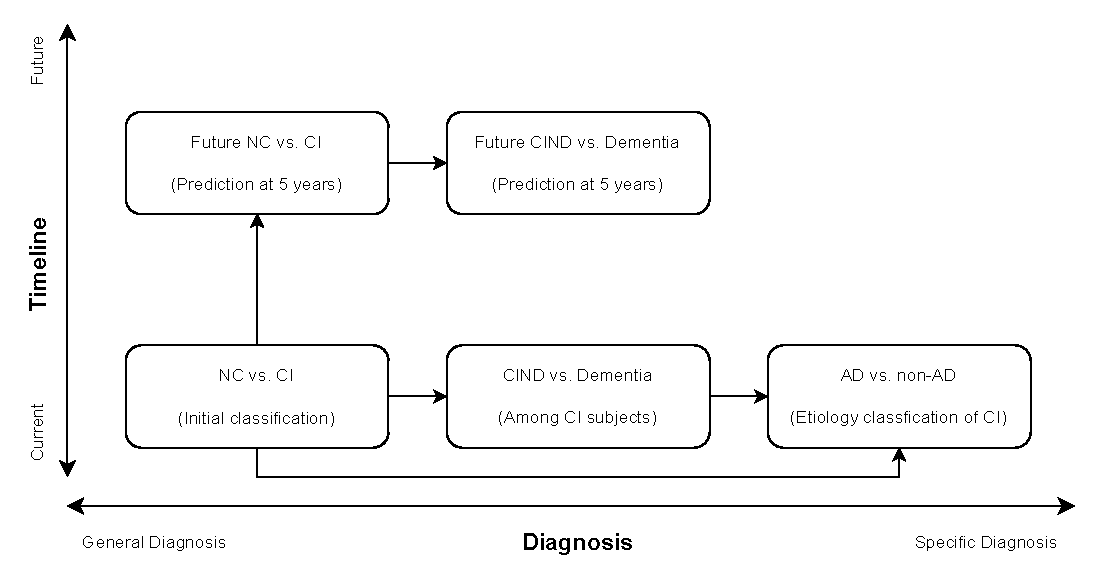
\includegraphics[width=\textwidth]{figures/classification-tasks.pdf}
    \caption[The segmentation of the classification problem into five tasks using hierarchical classification strategy]{The segmentation of the classification problem into five tasks using a hierarchical classification strategy\hl{, organised along two dimensions: the timeline (current versus future) and the diagnosis (general versus specific), and connected by arrows that represent common diagnosis paths in clinical practice}}
    \label{fig:classification-tasks}
\end{figure}

For the current cognitive status classification, both input features and target labels were derived from the ' baseline visit of the subjects. The classification task was then divided into two hierarchical tasks. First, a model was trained to differentiate NC subjects from all CI subjects. Second, another model was trained only on impaired subjects to further classify them as CIND or dementia. \hl{Demographic comparisons of the three cognitive statuses are summarized in} Table~\ref{table:ci-classification-demographics} \hl{for NACC UDS dataset and} Table~\ref{table:adni-classification-demographics} \hl{for ADNI dataset.}

\begin{table}[htbp]
\centering
\caption{Demographic characteristics of the NACC UDS subjects used in the current cognitive status classification tasks}
\label{table:ci-classification-demographics}
\footnotesize
\begin{tabular}{lcccc}
\toprule
 & \multicolumn{4}{c}{Cognitive Status} \\
\cmidrule{2-5}
Characteristic & NC & CIND & Dementia & Total \\
 & (n=21,919) & (n=14,445) & (n=17,151) & (N=53,515) \\
\midrule
\textbf{Age, years} \\
\quad Mean ± \acrshort{SD} & 69.4 ± 10.8 & 71.9 ± 9.4 & 72.3 ± 10.4 & 71.0 ± 10.4 \\
\\
\textbf{Sex} \\
\quad Female & 14,361 (65.5\%) & 7,468 (51.7\%) & 8,879 (51.8\%) & 30,708 (57.4\%) \\
\quad Male & 7,558 (34.5\%) & 6,977 (48.3\%) & 8,272 (48.2\%) & 22,807 (42.6\%) \\
\\
\textbf{Education, years} \\
\quad Mean ± SD & 15.8 ± 3.0 & 15.2 ± 3.4 & 14.5 ± 3.7 & 15.2 ± 3.4 \\
\\
\textbf{Marital Status} \\
\quad Married & 12,819 (58.5\%) & 9,050 (62.7\%) & 11,877 (69.2\%) & 33,746 (63.1\%) \\
\quad Other & 9,100 (41.5\%) & 5,395 (37.3\%) & 5,274 (30.8\%) & 19,769 (36.9\%) \\
\bottomrule
\end{tabular}
\end{table}

\begin{table}[htbp]
\centering
\caption{Demographic characteristics of the ADNI subjects used in the current cognitive status classification task}
\label{table:adni-classification-demographics}
\footnotesize
\begin{tabular}{lcccc}
\toprule
 & \multicolumn{4}{c}{Cognitive Status} \\
\cmidrule{2-5}
Characteristic & NC & CIND & Dementia & Total \\
 & (n=514) & (n=832) & (n=429) & (N=1,775) \\
\midrule
\textbf{Age, years} \\
\quad Mean ± \acrshort{SD} & 73.4 ± 6.4 & 73.3 ± 7.5 & 74.5 ± 7.5 & 73.6 ± 7.2 \\
\\
\textbf{Sex} \\
\quad Female & 274 (53.3\%) & 327 (39.3\%) & 184 (42.9\%) & 785 (44.2\%) \\
\quad Male & 240 (46.7\%) & 505 (60.7\%) & 245 (57.1\%) & 990 (55.8\%) \\
\\
\textbf{Education, years} \\
\quad Mean ± SD & 16.4 ± 2.6 & 16.1 ± 2.8 & 15.4 ± 2.9 & 16.0 ± 2.8 \\
\\
\textbf{Marital Status} \\
\quad Married & 335 (65.2\%) & 633 (76.1\%) & 360 (83.9\%) & 1,328 (74.8\%) \\
\quad Other & 179 (34.8\%) & 199 (23.9\%) & 69 (16.1\%) & 447 (25.2\%) \\
\bottomrule
\end{tabular}
\end{table}

The same hierarchical structure was designed for the early prediction of future cognitive status. However, specific criteria were applied for the inclusion of subjects for these prediction tasks. Only subjects with a baseline visit and a follow-up visit five years later were included. The input data for these tasks were extracted from the baseline visits, whereas the target classes were based on the diagnosis at a follow-up visit made approximately five years later. To accommodate for variability in visit timelines, a time frame of six months before or after the five-year mark was used. Subjects whose follow-up visits did not occur within this time frame were excluded. This future prediction task was also divided into two binary tasks: one for predicting future NC versus future CI status, and a second to differentiate future CIND from future dementia. Table~\ref{table:ci-prediction-demographics} and Table~\ref{table:adni-prediction-demographics} \hl{summarize the demographic characteristics of the subjects included in the future cognitive status prediction tasks for the NACC UDS and ADNI datasets, respectively.}

\begin{table}[htbp]
\centering
\caption{Demographic characteristics of the NACC UDS subjects used in the five years cognitive status prediction tasks}
\label{table:ci-prediction-demographics}
\footnotesize
\begin{tabular}{lcccc}
\toprule
 & \multicolumn{4}{c}{Cognitive Status} \\
\cmidrule{2-5}
Characteristic & NC & CIND & Dementia & Total \\
 & (n=6,612) & (n=2,334) & (n=3,399) & (N=12,345) \\
\midrule
\textbf{Age, years} \\
\quad Mean ± SD & 70.2 ± 9.2 & 72.9 ± 9.2 & 72.6 ± 9.6 & 71.4 ± 9.4 \\
\\
\textbf{Sex} \\
\quad Female & 4,354 (65.8\%) & 1,208 (51.8\%) & 1,715 (50.5\%) & 7,277 (58.9\%) \\
\quad Male & 2,258 (34.2\%) & 1,126 (48.2\%) & 1,684 (49.5\%) & 5,068 (41.1\%) \\
\\
\textbf{Education, years} \\
\quad Mean ± SD & 16.1 ± 2.8 & 15.6 ± 3.2 & 15.2 ± 3.5 & 15.8 ± 3.1 \\
\\
\textbf{Marital Status} \\
\quad Married & 3,918 (59.3\%) & 1,426 (61.1\%) & 2,522 (74.2\%) & 7,866 (63.7\%) \\
\quad Other & 2,694 (40.7\%) & 908 (38.9\%) & 877 (25.8\%) & 4,479 (36.3\%) \\
\bottomrule
\end{tabular}
\end{table}

\begin{table}[htbp]
\centering
\caption{Demographic characteristics of the ADNI subjects used in the five years cognitive status prediction task}
\label{table:adni-prediction-demographics}
\footnotesize
\begin{tabular}{lcccc}
\toprule
 & \multicolumn{4}{c}{Cognitive Status} \\
\cmidrule{2-5}
Characteristic & NC & CIND & Dementia & Total \\
 & (n=348) & (n=309) & (n=169) & (N=826) \\
\midrule
\textbf{Age, years} \\
\quad Mean ± \acrshort{SD} & 72.2 ± 6.5 & 72.3 ± 7.2 & 73.4 ± 6.4 & 72.4 ± 6.8 \\
\\
\textbf{Sex} \\
\quad Female & 190 (54.6\%) & 117 (37.9\%) & 72 (42.6\%) & 379 (45.9\%) \\
\quad Male & 158 (45.4\%) & 192 (62.1\%) & 97 (57.4\%) & 447 (54.1\%) \\
\\
\textbf{Education, years} \\
\quad Mean ± SD & 16.7 ± 2.5 & 16.1 ± 2.7 & 15.9 ± 2.8 & 16.3 ± 2.7 \\
\\
\textbf{Marital Status} \\
\quad Married & 233 (67.0\%) & 230 (74.4\%) & 137 (81.1\%) & 600 (72.6\%) \\
\quad Other & 115 (33.0\%) & 79 (25.6\%) & 32 (18.9\%) & 226 (27.4\%) \\
\bottomrule
\end{tabular}
\end{table}

\newpage
The data selection method for future cognitive status prediction tasks is illustrated in Figure~\ref{fig:prediction-data-selection}. Each row in the diagram represents visits made by a single subject. Subject's visits are donated with boxes. A selection window was set between 54 and 66 months (4.5 to 5.5 years) from the baseline visit (initial visit). Subjects who made a visit within the selection window were selected (denoted with a tick symbol). Subjects were excluded if they did not make a visit within the selection window (denoted with a cross sign). For selected subjects, data from the baseline visit are used as input data (boxes with ``IN''), and target classes are obtained from the visits made within the selection window (boxes with ``T''). It can be noticed that the selection of the subjects depends solely on the availability of visits made within the selection window, regardless of the number of visits made and the regularity of the time interval between visits. 

\begin{figure}[ht]
    \centering
    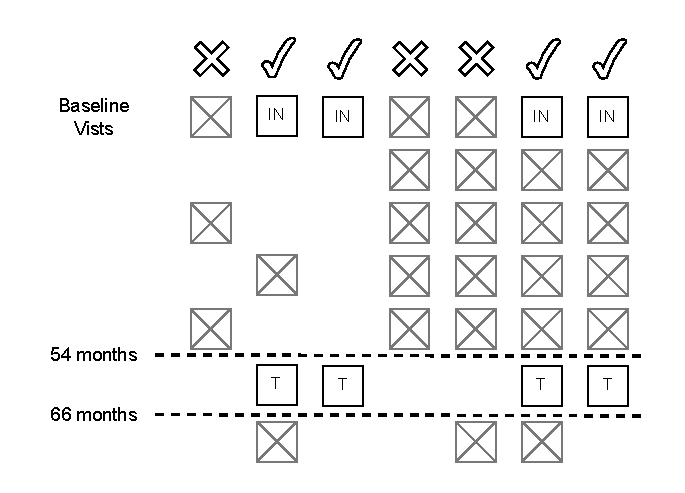
\includegraphics[width=0.8\linewidth]{figures/prediction-data-selection.pdf}
    \caption[The data selection method for the prediction of future cognitive status]{The data selection method for the prediction of future cognitive status\hl{, based on a 4.5--5.5 year selection window from the baseline visit. A tick symbol indicates included subjects, while a cross symbol indicates excluded subjects. Box labels ``IN'' and ``T'' denote input data and target classes, respectively.}}
    \label{fig:prediction-data-selection}
\end{figure}

It should be noted that cognitive status in the NACC UDS is classified as normal cognition, MCI, impaired-not-MCI, or dementia. Impaired-not-MCI refers to subjects who show cognitive difficulties but do not satisfy the clinical criteria for MCI. In this research work, MCI and impaired-not-MCI have been combined into a single class that represents CIND. Impaired-not-MCI cases are not treated as normal because they could indicate a risk of future progression to severe cognitive impairment. On the other hand, having impaired-not-MCI as a separate class could increase the complexity of the classification problem. This approach aligns with the objectives of this study to develop cost-effective early prediction models of CI. Compared to the literature, most of the studies that use NACC UDS do not clearly state how they address impaired-not-MCI cases \cite{abbas2024Explainable, Pang2023Predicting, Ren2023Improving}. These studies classify cognitive status as NC, MCI, and dementia. 

In addition to the cognitive status classification, another classification task is implemented to classify the subtype of current CI. The model in this task classifies the etiology of CI as AD versus other non-AD etiologies. The input data and the target classes are obtained from baseline visits of subjects with CIND or dementia. Subjects with normal cognition are not included in this classification task. Demographic differences between AD subjects and non-AD subjects are summarized in Table~\ref{table:ci-type-demographics}.

\begin{table}[htbp]
\centering
\caption{Demographic characteristics of the NACC UDS subjects used in the cognitive impairment subtype classification task}
\label{table:ci-type-demographics}
\footnotesize
\begin{tabular}{lcccc}
\toprule
 & \multicolumn{3}{c}{Cognitive Impairment Type} & \\
\cmidrule{2-4}
Characteristic & AD & Non AD & Total \\
 & (n=18,201) & (n=13,441) & (N=31,642) \\
\midrule
\textbf{Age, years} \\
\quad Mean ± SD & 73.7 ± 9.6 & 70.0 ± 10.1 & 72.1 ± 10.0 \\
\\
\textbf{Sex} \\
\quad Female & 9,923 (54.5\%) & 6,448 (48.0\%) & 16,371 (51.7\%) \\
\quad Male & 8,278 (45.5\%) & 6,993 (52.0\%) & 15,271 (48.3\%) \\
\\
\textbf{Education, years} \\
\quad Mean ± SD & 14.7 ± 3.7 & 14.9 ± 3.5 & 14.8 ± 3.6 \\
\\
\textbf{Marital Status} \\
\quad Married & 12,162 (66.8\%) & 8,794 (65.4\%) & 20,956 (66.2\%) \\
\quad Other & 6,039 (33.2\%) & 4,647 (34.6\%) & 10,686 (33.8\%) \\
\bottomrule
\end{tabular}
\end{table}

The use of hierarchical binary classification has proven to produce a better classification accuracy compared to the multi-classification approach in studies related to dementia \cite{Ren2023Improving}. The complexity of the data that a single classifier needs to learn for multi-classification has been reduced by decomposing the data to simpler data domains. Furthermore, in imbalanced and overlapped domains, separating classes promotes focused feature selection, targeted data resampling, and tailored model tuning to improve classification performance. Additionally, this approach increases the clinical utility of classification models. Implementing staged classification mirrors the real-world diagnostic flow in which impairment is first diagnosed (normal vs. impaired) before the severity of impairment is identified. It also allows for the use of specialized models for specific use cases. Moreover, hierarchical binary classification supports the transparent and clinically meaningful interpretability of the model through an independent explanation of each decision stage.

In contrast, hierarchical binary classification has pitfalls that could affect the accuracy and interpretation of the outputs of multiple models. Classification at multiple levels could result in compound errors where misclassifications at the first level could impact the correctness of the downstream binary model. Additionally, combining the interpretation of the output of multiple models is necessary to gain an overall understanding of the subject's cognitive status. Not to mention the added workload and complexity in training, tuning, and evaluating multiple models. With these concerns in mind, the research methodology of this study was designed around the hierarchical binary classification approach because of its potential to improve classification performance and clinical practicality.

\section{Data Preprocessing}
Data preprocessing improves the quality of the data by cleaning, transforming, and organizing the raw data to be suitable for analysis. It is undeniably the most critical process for developing an accurate classification model. The quality of the data has a direct impact on the model performance, especially on imbalanced and overlapped data domains. As a result, significant effort and emphasis were dedicated to this phase of the research work. The primary objective of data preprocessing is to improve data quality and mitigate the impact of data irregularities, such as class imbalance and overlap. Class overlap measures were used to guide data preprocessing techniques and assess their effectiveness. In this research, data preprocessing can be categorized into data imputation, feature engineering, feature selection, and data resampling.

The initial raw data were extracted from the NACC UDS and ADNI datasets based on easily accessible data. According to the categorization by affiliated neurologists and neuropsychologists \cite{Ren2023Improving}, easily accessible data can be acquired quickly and efficiently without the need for specialized tools or advanced skills. A general practitioner can collect these data during primary care visits by conducting direct interviews with the subjects or their caregivers. These data include the subject's demographics, health and family history, behavioral surveys, and basic functional and cognitive tests. All of these data were classified as lower cost in a three-tiered categorization based on the cost required to obtain the associated information \cite{Ren2023Improving}. Refer to Table \ref{table:initial-uds-variables} in the appendix for more details of the initially selected accessible data variables.

\subsection{Data Imputation}
It is important to properly handle missing data to ensure model reliability and to prevent biases that may result from incomplete observations. In this study, data imputation was only applied to the NACC UDS dataset. Samples with missing values in the ADNI dataset were excluded to maintain the integrity of external testing and to avoid introducing differing imputation assumptions across datasets. Most of the missing data in the NACC UDS came from the nature of collecting data from multiple centers and utilizing different versions of data collection forms. Subjects or their informants were sometimes unable or unwilling to answer certain questions during the interview. Additionally, systematic missing data occurred due to skip patterns in the assessment protocol that prevented follow-up questions. It has been noticed that variables related to physical measurement, such as height and weight, comprise the highest percentage of missing data. This could be due to challenges in performing the assessment during telephone visits. The percentages of missing data in different NACC UDS forms for the data of all classification tasks are presented in Table \ref{table:miss-data} in the appendix.

The data imputation workflow consists of multiple steps. First, any data sample with 50\% or more missing values was removed. This limits the risk of excessive information loss against the potential distortion introduced by imputing very sparse samples. This method is applied and verified by other studies in the literature \cite{abbas2024Explainable, Vyas2022Identifying}. Second, the remaining missing values were imputed using appropriate statistical methods based on the type of variables. The mode is used for nominal variables, the median for ordinal variables, and the mean for continuous data. Refer to Table \ref{table:initial-uds-variables} in the appendix for the types of variables. The missing values of the derived variables, such as the total Geriatric Depression Scale score (NACCGDS) and the body mass index (NACCBMI), were recalculated using the imputed values of the source variables. Statistical imputation techniques were employed because the rate of missing values is small in addition to their simplicity, computational efficiency, and ability to maintain the central tendency of the dataset. This imputation method is commonly used by other studies that use the same dataset \cite{abbas2024Explainable, Wang2018Predictive}. To prevent data leakage, imputation parameters (the mode, median, and mean) were first fitted using only the training dataset and then applied to the missing data in the testing dataset. Finally, the values of the Functional Activities Questionnaire (\acrshort{FAQ}) required special attention. The “never did” category was retained as a valid value if it represented at least 3\% of observations. Treating "never did" as a valid value preserves meaningful differences in functional ability and enhances the integrity of the analysis. For instance, since many people have not filed taxes before, preserving a specific category better reflects their functional ability. These procedures were essential to maintain the quality of the data and support reliable downstream modeling in this research work.

\subsection{Feature Engineering}
Effective feature engineering is required to convert raw clinical data into informative input that improves the efficiency of the modeling process and enhances the performance of the model. Guided by statistical criteria and domain knowledge from the literature, systematic transformations were applied to categorical and continuous features.

The feature engineering process involved the alignment of data from the NACC UDS and ADNI datasets. Various categorical variables were found to be defined using different sets of categories across the two datasets. Therefore, an alignment of these categories was performed. For instance, the primary language variable in the NACC UDS dataset has been transformed to align with the categories in the ADNI dataset (English, Spanish, and others). This is done by aggregating other languages into one category. Other transformed demographic features include marital status and type of residence. Variables related to the subject's health history were converted to binary features by grouping inactive and active categories to indicate the presence of the condition. This binarization was required due to the low representation of these values and to align the NACC UDS dataset with the ADNI dataset. This alignment was a critical requirement to ensure data consistency, which was required for the external validation phase. \hl{Previous studies used similar alignment steps that successfully aligned the feature in the NACC UDS and ADNI datasets} \cite{abbas2024Explainable, Qiu2022Multimodal}. Additionally, as part of feature engineering, categorical features with a dominant category accounting for 97\% of the samples were excluded to prevent potential model bias and improve performance. Furthermore, some initially selected variables from the NACC UDS dataset were excluded because they are not available in the ADNI dataset. The excluded variables are listed in Table~\ref{table:excluded-dominant-features} in the appendix. \hl{These feature engineering choices were guided by statistical criteria and prior literature to minimize potential bias, although it is acknowledged that the alignment and binarization steps may cause a minor loss of information.}

In this research, the relationship between the features was calculated and examined. Since the dataset consists of a mixture of continuous and categorical features, suitable correlation methods were used depending on the type of the features. Cramer's V was used to calculate the correlation between categorical features and Pearson was utilized to measure correlation between the continuous features. Additionally, the correlation ratio for multiple categorical and continuous feature pairs was calculated. An absolute correlation ratio above 0.70 was considered high and was addressed by merging the correlated features or excluding the less informative features. Features with moderate correlations were managed during the subsequent feature selection.

Finally, proper encoding and scaling methods were used to maintain the integrity of the original data while preparing the data for modeling. Categorical variables were encoded according to their characteristic. One-hot encoding was applied to nominal features, whereas ordinal features were encoded using ordinal encoding to preserve the order of categories. Continuous variables were scaled with a robust scaler to reduce the impact of outliers. \hl{To prevent data leakage, the encoding and scaling parameters were fitted on the training dataset only and then applied to the testing dataset.}
% TODO: (optional) draw figure that show how features flow from initial set, to ADNI available selection, to feature selection (refer to 41598_2024_51985_MOESM1_ESM.pdf)

In the next sections, feature selection and data resampling to handle class imbalance and overlap are discussed. The implementation of these two important steps of data preprocessing was guided by the characteristics of class overlap. The following section provides a detailed discussion on the problem of class overlap.

\subsection{Class Overlap} \label{class-overlap-section}
Class overlap is a significant issue that occurs when examples from different classes are located in the same region of the data. This makes it harder for models to set clear decision boundaries. The problem is exacerbated in imbalanced domains, where the scarce minority class examples may primarily reside in regions shared with the majority class, making their classification significantly more difficult. In overlapped and imbalanced domains, addressing class imbalance is often insufficient without handling class overlap. Classification performance is significantly affected by the presence of class overlap even with balanced datasets \cite{Pattaramon2021On}

There are several factors that can lead to class overlap \cite{Santos2022Joint}. An important reason is inherent ambiguity, which means that some classes are very similar and difficult to differentiate. Another factor is the limited feature representation, which means that the measured features do not pick up enough of the differences between classes. Additionally, diagnosis mistakes or labeling errors can cause overlapping instances and create complex class boundaries. All of these factors could apply to the datasets used in this study.

Class overlap appears in various forms and can be attributed to different underlying causes and characteristics of the data \cite{Santos2023Unifying}. Therefore, it is regarded as a heterogeneous concept. Identifying class overlap is crucial because it allows for a more detailed understanding of the problem. Different types of overlap may require different approaches to mitigate. Additionally, a comprehensive view of class overlap enables researchers to develop more targeted and effective solutions \cite{Santos2023Unifying}. The identification of class overlap is done using various methods that aim to characterize and quantify the ambiguous regions. These identification methods often lead to different representations of class overlap. Each representation highlights a particular aspect of the phenomenon. Common representations include:
\begin{itemize}
\item \textbf{Feature Overlap}: This refers to the overlap in the distribution of individual features between classes.
\item \textbf{Instance-Level Overlap}: This focuses on specific data points that lie in ambiguous regions, often referred to as "borderline" or "noisy" instances. It is based on characteristics of local data (local information).
\item \textbf{Structural Overlap}: This considers the overlap in the underlying data structure or clusters. It is based on geometrical and graph-based properties of the data. This may indicate that class clusters are not well separated in the data space.
\end{itemize}
\vspace{2em}

% It is important to note that merely measuring the class overlap degree (a single numerical value indicating the extent of overlap) is often not sufficient \cite{Santos2022Joint}. This is because a single degree measure might miss the specific nature or cause of the overlap. For instance, two datasets might have the same degree of overlap but suffer from entirely different types of overlap (e.g., one due to inherent ambiguity, another due to noisy labels). A single metric is not capable of capturing the heterogeneity of the problem or providing insights about the class overlap, such as which features or instances are impacted. Therefore, understanding the different representations and causes of overlap is essential for effective analysis and resolution.

There are available measures that are used to quantify class overlap \cite{Santos2022Joint}. Each measure offers different insights into the type of overlap. It is necessary to use different class overlap measures to build a thorough understanding of how classes interact. The measures listed below were employed in this study to obtain information about the class overlap. These insights were used to design optimized techniques, such as feature selection and data resampling. These class overlap measures cover various representations of the overlapped domains, including feature overlap, instance-level overlap, and structural overlap.

\begin{itemize}
\item \textbf{Maximum Fisher's Discriminant Ratio (\acrshort{F1})}: This is a feature overlap measure. It is used to define the discriminative power of individual features \cite{Lorena2019How}. For its mechanism, Fisher's discriminant ratio, which is based on class means and variances, is computed for each feature. The maximum value found among all the features is then used. Typically, the inverse of this value is taken, where higher values indicate more overlap.

\item \textbf{Borderline Examples}: This measure is associated with the overlap of instances. It quantifies the percentage of data points that are located near the decision boundary between classes. Data examples are categorized according to their local neighborhood (e.g., $k=5$). An example is designated as "borderline" if a specific number of its neighbors, such as two or three, belong to the opposite class. The final measure is the total count of these examples normalized by the size of the dataset.
\item \textbf{k-Disagreeing Neighbors (\acrshort{kDN})}: This measure is used to measure the local overlap for an individual instance (instance-level overlap) \cite{Smith2013Instance}. For each instance, the percentage of k-nearest neighbors that do not belong to the same class as the instance is calculated. The value is used to indicate whether the data point is in a safe or overlapped region. This can be averaged over all samples to produce a global measure.
\item \textbf{Fraction of Borderline Points (\acrshort{N1})}: This measures structural overlap by assessing the complexity of the decision boundary \cite{Ho2002Complexity}. It indicates how deeply the classes are intertwined. For its mechanism, a minimum spanning tree (\acrshort{MST}) is constructed for the entire dataset. The measure is the proportion of examples in the dataset that are connected by an edge in the MST to an example from the opposite class.
\end{itemize}
\vspace{2em}

These class overlap measures are discussed in more detail in a recent review \cite{Santos2022Joint}. The following sections explain how insights from these class overlap measures were used to guide the feature selection and data resampling methods in this study.

\subsection{Ensemble Feature Selection}
In the context of developing cost-effective and accessible predictive models for CI, feature selection constitutes a critical step in the development of robust and generalizable machine learning models. Selecting the most informative subset from a larger pool of features is essential to mitigate high dimensionality, reduce the risk of overfitting, and improve model interpretability and computational efficiency. All of these advantages are aligned with the objectives of this study. \hl{In particular, reducing the feature subset is one of the main components that promote the cost-effectiveness of the developed models, since fewer features lower the data collection and computational costs.} The feature selection method in this study was designed based on a two-step automated approach. The strategy combines an ensemble of diverse feature ranking methods with a class overlap-driven thresholding technique. These two steps are explained in the following subsections. Refer to Figure~\ref{fig:feature-selection} for an overview of the proposed feature selection method.

\begin{figure}
    \centering
    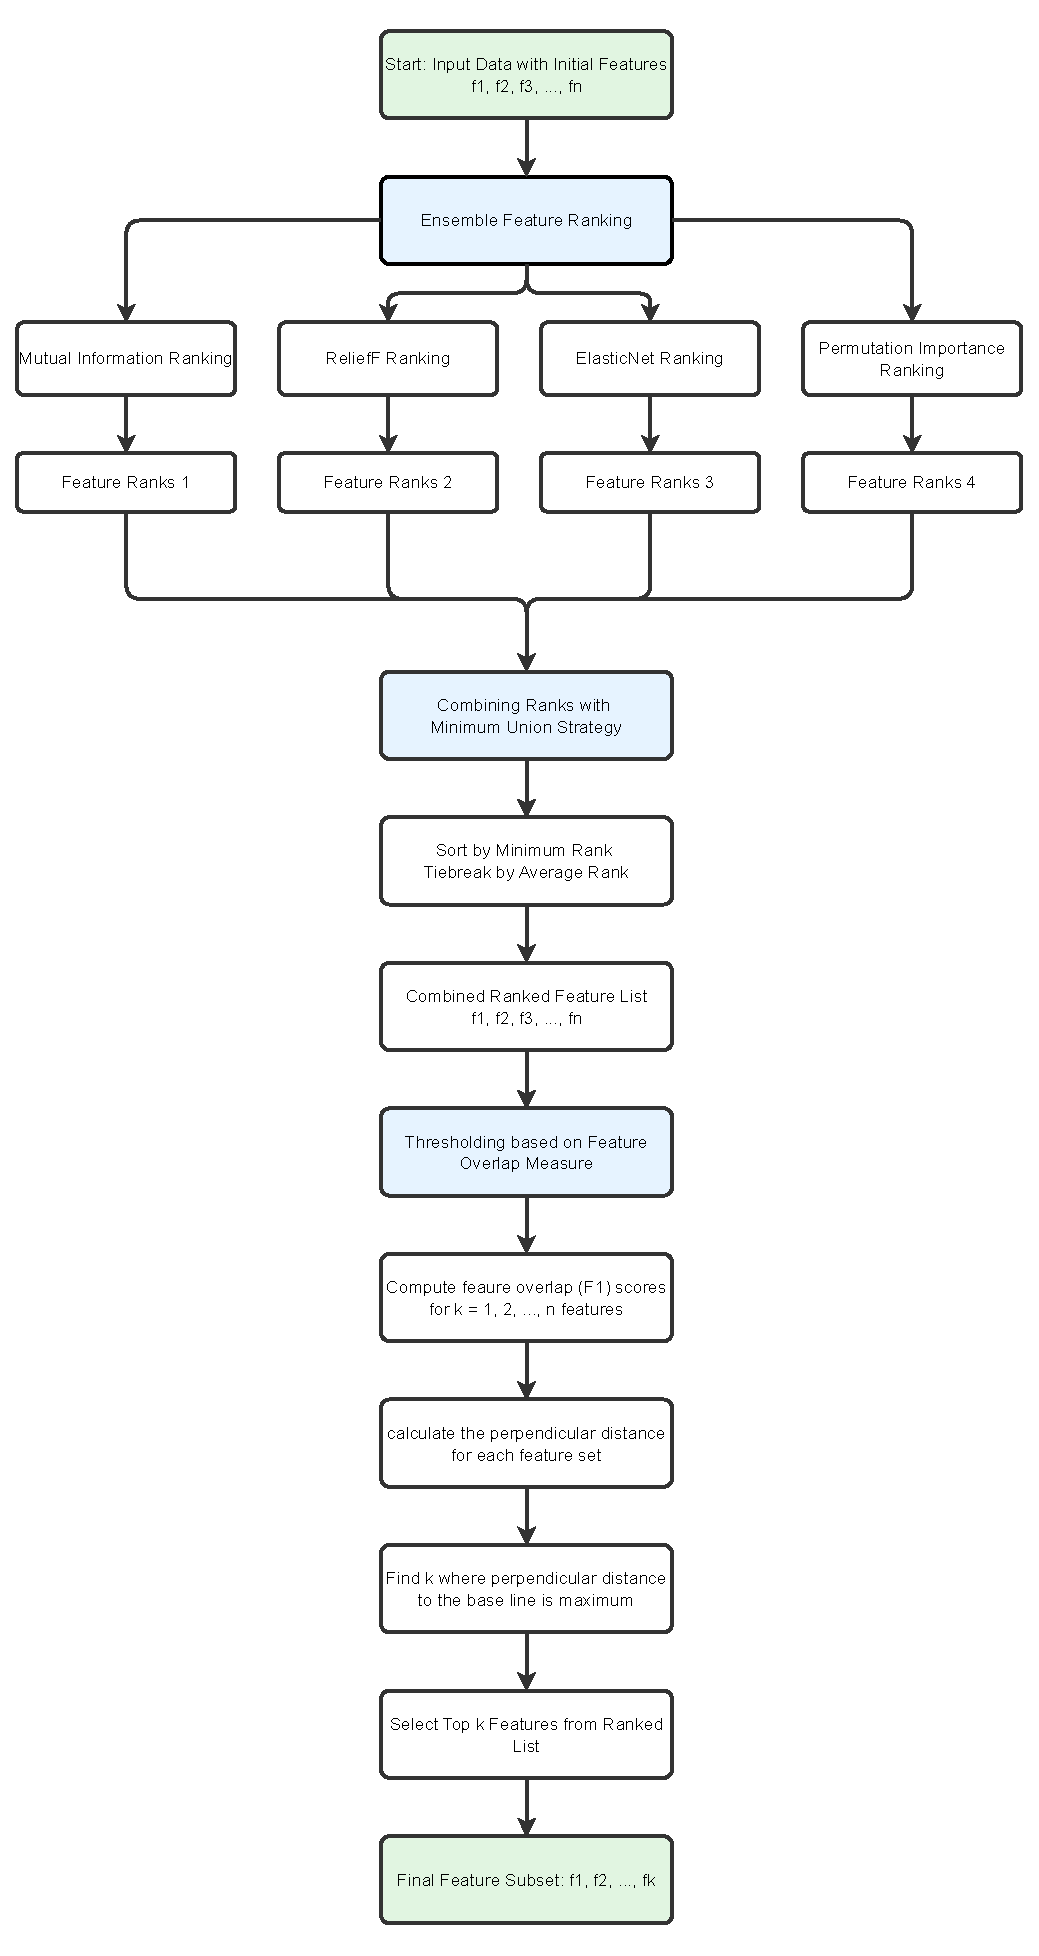
\includegraphics[width=0.7\textwidth]{figures/feature-selection-method.pdf}
    \caption[Flowchart of the proposed ensemble feature selection method]{Flowchart of the proposed ensemble feature selection method\hl{. It combines multiple feature ranking methods and a class overlap-driven thresholding technique to select the most informative features}}
    \label{fig:feature-selection}
\end{figure}

\subsubsection{Combination Step: Aggregating Feature Rankings}
The objective of this step is to combine the feature rankings obtained from various feature selection methods into a single ranking. Four feature selection methods have been utilized: mutual information \cite{Peng2005Feature}, ReliefF \cite{Robnik-ikonja2003Theoretical}, elastic net \cite{Zou2005Regularization}, and permutation importance using random forest. Each of these methods follows a different approach to select informative features, including filter, wrapper, and embedded techniques. These approaches have different sensitivities to data characteristics such as noise, feature correlation, and non-linear interactions. As an example, Mutual Information and ReliefF are effective at detecting non-linear relationships, whereas elastic net is effective at feature correlation. Therefore, the use of this diverse ensemble approach ensures a comprehensive evaluation of feature importance from multiple analytical perspectives. The results of the feature ranking methods were analyzed using Spearman correlation to ensure that these feature selection methods are complementary and do not highly overlap.
% TODO: table #t comparing the feature selection methods

The minimum union method was utilized to combine these individual rankings into a unified list. The features were added to the unified list based on their minimum rank across all four methods. The average of the ranks of a feature across the four methods was used in cases where multiple features have the same minimum rank. This method resulted in a strong and stable sorted list of features, which was used by the following step to identify the optimal subset of features. Figure~\ref{fig:minimum-union} illustrates the proposed feature ranking method. 

\hl{The ensemble feature ranking approach is adopted to avoid biased or unstable results that can be obtained by using a single feature ranking method, particularly in high-dimensional clinical and neuropsychological data. This approach has been successfully employed across predictive modeling studies in the literature. For example, \mbox{\cite{Pereira2018Neuropsychological}} combined multiple filter and embedded methods to predict the conversion from MCI to AD. It was found that combining subsets from different selection methods creates a consensus that improves the robustness, stability, and generalizability of the selected features. Furthermore, this finding was confirmed by another study } \cite{Spooner2023Ensemble} \hl{that applied ensemble feature selection with data-driven thresholding on Alzheimer's disease datasets, including the ADNI cohort.}

\begin{figure}[ht]
    \centering
    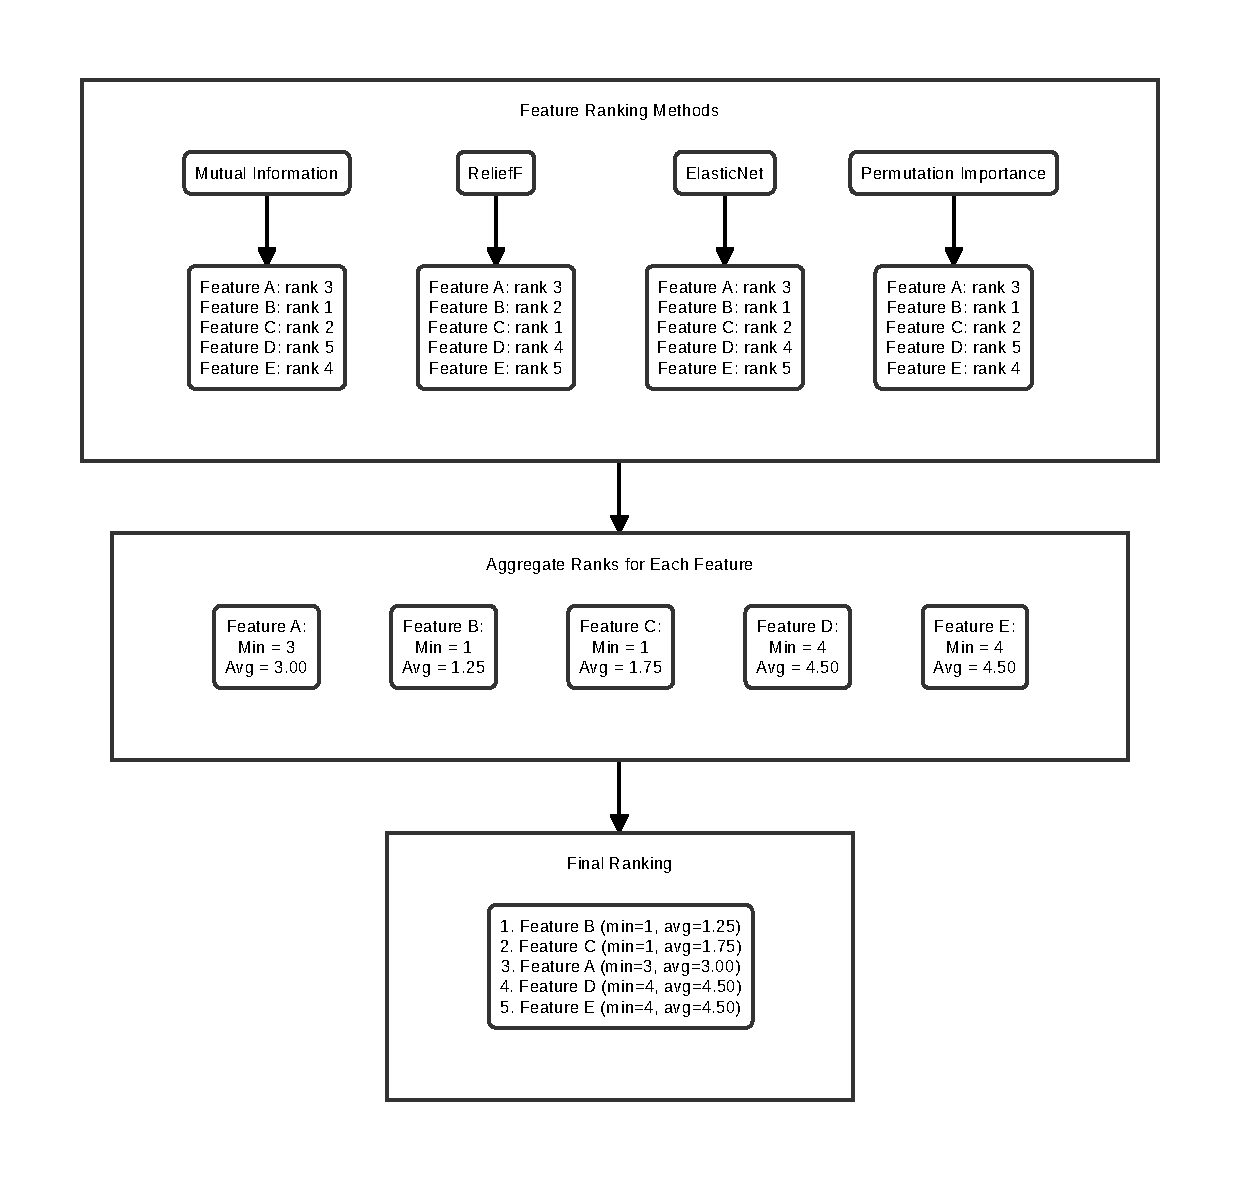
\includegraphics[width=\textwidth]{figures/minimum_union_diagram.pdf}
    \caption[Illustration of the minimum union feature ranking aggregation method]{Illustration of the minimum union feature ranking aggregation method\hl{. The method merges four separate feature rankings into one unified ranking by their minimum rank}}
    \label{fig:minimum-union}
\end{figure}

\subsubsection{Thresholding Step: Selecting Features Based on Class Overlap Measures}
The second step addresses the challenge of determining the optimal number of features, denoted as \textit{k}, to be retained from the ranked features. To do this, a class overlap measure is used as a dynamic thresholding mechanism, instead of random feature counts or levels of statistical significance. Using the class overlap measure as a threshold selects the optimal set of features that minimizes the inherent complexity of the data. As a result, it facilitates more effective model training and improves predictive performance.

The process begins by iteratively constructing subsets of features, starting with the top-ranked feature and progressively adding one feature at a time from the ranked list of features from the previous combination step. For each subset of \textit{k} features, the class overlap was quantified using a modified F1 measure of all features in the subset. The F1 measure was computed by first calculating the Fisher's discriminant ratio for each feature in the subset. This calculation is presented in equation \eqref{eq:fisher-ratio}. After that, the inverse of the summation of these values was obtained, as shown in equation \eqref{eq:f1-measure-feature-set}. This inverse ensures that feature subsets with better overall discriminative power (higher individual discriminant ratios) result in smaller F1 values. On the other hand, subsets with poorer class separability produce larger F1 values. Consequently, during feature selection, the objective was to minimize the F1 value to identify the set of features that provides the most effective class discrimination.

\newpage

\begin{equation}
    F1_i = \frac{\sum_c p(c) \times (\mu_c - \mu)^2}{\sum_c p(c) \times \sigma_c^2}
    \label{eq:fisher-ratio}
\end{equation}
Where:
\begin{itemize}
    \item $p(c)$ = proportion of samples in class $c$
    \item $\mu_c$ = mean value of feature $x_i$ for class $c$
    \item $\mu$ = overall mean of feature $x_i$ across all samples
    \item $\sigma_c^2$ = variance of feature $x_i$ within class $c$
\end{itemize}
\vspace{2em}

The Fisher's discriminant ratio of a single feature ($F1_i$) is calculated by computing the ratio of between-class scatter (numerator) to within-class scatter (denominator). Features that exhibit larger between-class separation relative to their within-class variance yield higher discriminant ratios. This indicates that the feature has better class separability.

\begin{equation}
    F1(S) = \frac{1}{\sum_{i=1}^{k} F1_i}
    \label{eq:f1-measure-feature-set}
\end{equation}
Where:
\begin{itemize}
    \item $F1(S)$ = the F1 value for feature set $S$
    \item $k$ = the total number of features in the feature set $S$
    \item $F1_i$ = the Fisher's discriminant ratio of feature $i$ in the feature set $S$
\end{itemize}
\vspace{2em}

A distance-based method was used to determine the optimal set of features $S$ to select. The method is presented in equation \eqref{eq:elbow-method}. A curve is constructed by plotting the F1 values $F1(S)$ on the y-axis against the number of features $k$ on the x-axis. Each set of features is represented with a point on the curve that corresponds to its F1 value and the number of features. The perpendicular distance from each point on the curve to the line connecting the first and last points is calculated. The optimal set of features is indicated by the point with the maximum distance from this line. This optimal point is representative of the configuration where adding more features results in diminishing improvements in class separability. Using this method, a balance is achieved between model simplicity (fewer features) and reduced class overlap (a minimized F1 value).

\begin{equation}
    k_{optimal} = \arg\max_{i} \frac{|(p_n - p_1) \times (p_1 - p_i)|}{||p_n - p_1||}
    \label{eq:elbow-method}
\end{equation}
Where:
\begin{itemize}
    \item $p_1 = (k_1, F1(S_1))$ which is the point coordinates of the first feature set $S_1$ (including only the top ranked feature)
    \item $p_n = (k_n, F1(S_n))$ which is the point coordinates of the last feature set $S_n$ (including all the features)
    \item $p_i = (k_i, F1(S_i))$ which is the point coordinates of the $i$ feature set $S_i$
    \item $k_{optimal}$ -- optimal number of features at the point with maximum perpendicular distance
\end{itemize}
\vspace{2em}

\hl{The proposed approach of using an automatic data-driven threshold for feature selection was reviewed by} \cite{Santos2023Unifying}. \hl{It was highlighted that the utilization of data complexity measures is currently recognized as an effective strategy to guide feature selection and address class overlap in complex datasets.} \cite{FU2020Feature} \hl{proved that the selection of features based on the minimization of class overlap improves the sensitivity, the mean G and the classification performance in imbalanced domains. Similarly,} \cite{HU2022Attribute} \hl{demonstrated that selecting features that reduce the degree of class overlap effectively eliminates redundant features and produces high classification accuracies compared to other feature selection methods. The proposed feature selection method was inspired by} \cite{Seijo-Pardo2019developing} \hl{work. In their study, data complexity measures, such as the Maximum Fisher's Discriminant Ratio, were utilized to evaluate automatic cutoffs for ensemble feature rankings. The experimental results concluded that these automatic data-driven thresholds generally outperform traditional fixed-percentage thresholds. Although these specific studies were not conducted within the domain of cognitive impairment, their promising results encourage evaluating this data-driven approach with the clinical data of this research.}

The feature selection process was carried out on the internal cross-validation of each classification task. The set of features selected by this method was used to train a random forest (\acrshort{RF}) model with stratified cross-validation. RF was selected because it gives stable performance across different feature subsets without the need for hyperparameter tuning. The performance of the RF model was compared with the performance of models trained with the initial set of features and features selected by the Boruta method. This step is important in assessing the effectiveness of the proposed feature selection method compared to the baseline and a robust and commonly used feature selection method. This comparative evaluation was conducted using a fitness function \cite{Cano2003Using}. The fitness function provides a unified metric that balances classification accuracy with the complexity of the feature set. The fitness function is defined in equation \eqref{eq:fitness-function}.

\begin{equation}
    f = \alpha \times G_{mean} + (1 - \alpha) \times \left(1 - \frac{k}{d}\right)
    \label{eq:fitness-function}
\end{equation}
where:
\begin{itemize}
    \item $f$ is the fitness value
    \item $G_{mean}$ geometric mean to measure the model performance
    \item $\alpha$ is the weighting parameter (set as 5/6)
    \item $k$ is the number of selected features
    \item $d$ is the total number of initial features
\end{itemize}
\vspace{2em}

% This strategic approach of feature selection not only improves the predictive performance by reducing class overlap but also aligns with the broader objective of creating cost-effective models that are practical for deployment in resource-constrained clinical settings.

\subsection{Hybrid Data Resampling}
Class overlap is widely recognized as one of the most harmful issues for classification, especially in imbalanced data domains \cite{Santos2022Joint}. The existence of these two factors creates complex and challenging data domains for traditional and efficient classification models to learn. Models are often biased towards the majority class and consequently have a higher rate of misclassified minority class examples. The primary objective of the data resampling process in this study is to mitigate this bias. As a result, the resampled training data should increase the classification accuracy of the minority class (which is usually the class of interest) and lead to more balanced predictive performance between both classes. \hl{The hybrid data resampling is also a key component for developing cost-effective models, since improving the data quality reduces the need for complex and computationally expensive models.}

The selection of the most appropriate resampling method for a given classification problem can be difficult. The effectiveness of the applied technique is highly dependent on the underlying characteristics of the data. Rather than applying a generic data resampling, this study utilized a set of class overlap measures as a form of meta-knowledge to systematically guide the choice of the suitable data resampling method. The proposed methodology is illustrated in Figure~\ref{fig:data-resampling}. The process starts by measuring the class overlap on the training dataset. It measures the borderline examples and uses kDN to assess local class overlap and N1 to evaluate structural class overlap. Refer to section \ref{class-overlap-section} to learn more about these measures. The measures were interpreted to identify the specific nature and location of the overlapped regions. This insight was then used to design the suitable data resampling technique to handle the defined class overlap.

\begin{figure}[ht]
    \centering
    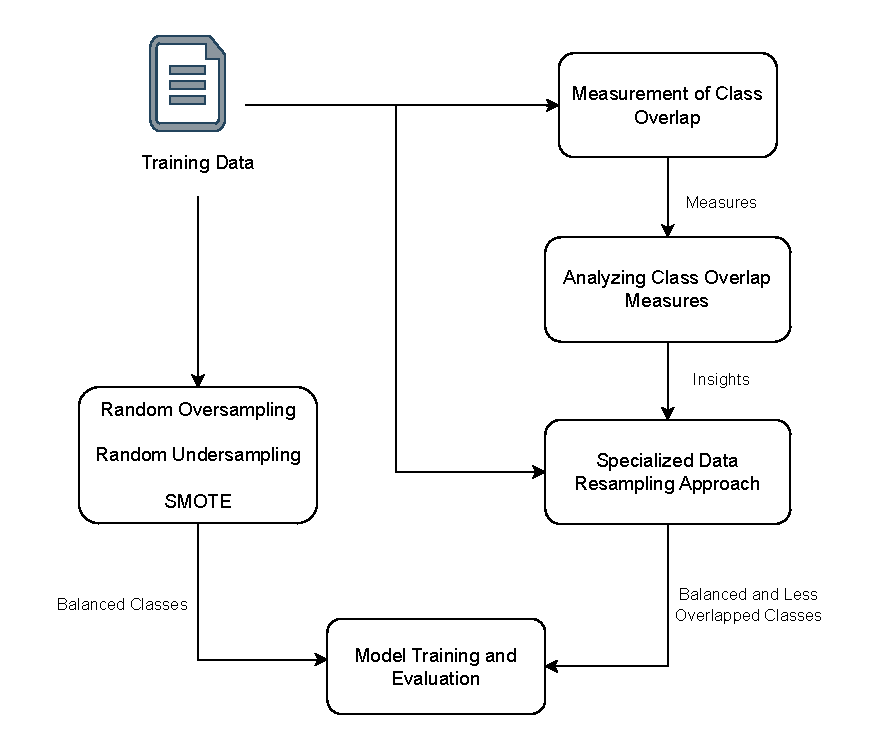
\includegraphics[width=\textwidth]{figures/data-resampling-diagram.pdf}
    \caption{Specialized data resampling approach guided by class overlap measures}
    \label{fig:data-resampling}
\end{figure}

The proposed methodology uses a hybrid data resampling approach, which combines cleaning-based and oversampling methods to address a particular aspect of class overlap. For the cleaning-based component, the Edited Nearest Neighbor (\acrshort{ENN}) method was used \cite{Wilson1972Asymptotic}. ENN works by removing data points from both classes that are considered noisy or mislabeled. It works by checking nearest neighbors of each data point. Data points were removed if the majority of their neighbors belong to a different class. This step helps to clean up the data by removing examples that fall on the wrong side of the decision boundary. Thus, it reduces noise and class overlap. 

The choice of the oversampling method depends on the region of class overlap. The K-means Synthetic Minority Over-sampling Technique (\acrshort{KMeansSMOTE}) \cite{Douzas2018Improving} was used to handle structural class overlap by boosting the safe and sparse regions of the minority class. It uses k-means clustering to group similar minority class instances together and then applies the Synthetic Minority Over-sampling Technique (\acrshort{SMOTE}) algorithm to generate new synthetic examples only within these specific clusters. This could create more meaningful and representative new data points, rather than producing synthetic examples in areas where they might be less helpful. The other oversampling method used in this study is \acrshort{BorderlineSMOTE} \cite{Han2005Borderline-SMOTE}. This method introduces new minority class examples in areas that are located around the decision boundary between different classes. This approach effectively strengthens the minority side of the overlapped border. As a result, it becomes easier for a model to accurately classify the minority class examples.

\hl{The combination of SMOTE with data cleaning methods, were proven by} \cite{Sharma2024Leveraging} \hl{to successfully reduce selection bias and significantly improve the classification accuracy of dementia subtypes. The hybrid data resampling approach was also evaluated in a critical review} \cite{Santos2022Joint}. \hl{Furthermore, the use of class overlap measures as metadata to guide data resampling is recognized by a recent review} \cite{Santos2023Unifying} \hl{as an effective strategy to overcome complex imbalanced data domains. The elimination of negative instances specifically in overlapping regions was proven by} \cite{Vuttipittayamongkol2020Improved} \hl{to significantly enhance sensitivity and overall classification performance in neurodegenerative disease datasets. Similarly,} \cite{Kraiem2021Selecting} \hl{demonstrated that the most effective data resampling strategy must be systematically guided by the intrinsic overlap and imbalance characteristics of the data rather than applying a universal method. Although some of these specific studies were not conducted using the identical clinical datasets of this research, the application of this approach is supported by their solid findings.}

The algorithm used to decide the suitable data resampling is presented in Algorithm \ref{alg:data-resampling}. Firstly, the imbalance ratio (\acrshort{IR}) and the class overlap measures (kDN and N1) are calculated based on the training dataset. After that, the algorithm checks for class overlap (kDN > 0.3 or N1 > 0.3) or moderate imbalance classes (IR > 2.0). Data resampling is skipped if neither class imbalance nor class overlap exists. On the other hand, if class overlap is found, ENN is applied to the training dataset to clear the overlapped instances and potential mislabeled examples in both classes. After that, the percentage of borderline examples for both classes is computed. This is followed by oversampling of the minority class using BorderlineSMOTE if the minority class is less represented around the class boundaries or KMeansSMOTE otherwise. This selection of the oversampling method ensures that the synthetic examples are added to sparse regions of the minority class. In cases where class imbalance exists without class overlap, oversampling is applied only without data cleaning using ENN.

\captionsetup[algorithm]{list=no}
\begin{algorithm}
\caption{Data Resampling Decision Algorithm}
\label{alg:data-resampling}
\begin{algorithmic}[1]
    \Require Training dataset $D$ with minority class $C_{min}$ and majority class $C_{maj}$
    \Ensure Resampled training dataset $D'$ or original training dataset $D$
    
    \State Compute $IR \leftarrow \frac{|C_{maj}|}{|C_{min}|}$
    \State Compute $kDN$ (k-Disagreeing Neighbours measure)
    \State Compute $N1$ (Fraction of Borderline Points measure)
    
    \If{$kDN > 0.3$ or $N1 > 0.3$ or $IR > 2.0$}
        \If{$kDN > 0.3$ or $N1 > 0.3$}
            \Comment{Apply ENN to $D$}
            \State $D \leftarrow ENN(D)$
        \EndIf

        \State Compute $BE_{min}$ (Percentage of Borderline Examples in $C_{min}$)
        \State Compute $BE_{maj}$ (Percentage of Borderline Examples in $C_{maj}$)
    
        \If{$BE_{min} < BE_{maj}$}
            \Comment{Apply BorderlineSMOTE to $D$}
            \State $D' \leftarrow \text{BorderlineSMOTE}(D)$
        \Else
            \Comment{Apply KMeansSMOTE to $D$}
            \State $D' \leftarrow \text{KMeansSMOTE}(D)$
        \EndIf
        \State \Return $D'$
    \Else
        \Comment{Skip data resampling}
        \State \Return $D$
    \EndIf
\end{algorithmic}
\end{algorithm}

To evaluate the chosen resampling method, the method is subsequently used to train a RF model in stratified cross-validation. RF was chosen because it demonstrates consistent behavior with imbalanced datasets. It also reduces the risk of overfitting, which could favor certain balancing approaches. The performance of the RF model is then compared with the baseline (without data resampling) and common resampling methods: random undersampling, random oversampling, and SMOTE \cite{Chawla2002SMOTE}. This evaluation assesses the geometric mean (\acrshort{G-mean}) and the recall of both binary classes. A data resampling method that improves the accuracy of the minority class and provides a balanced performance between both classes is selected. The data resampling methods were implemented using the imbalanced-learn library version 0.12.4 \cite{Lematre2016Imbalanced-learn}.

% By combining these two techniques, the hybrid method first cleans the data with ENN and then selectively generates new samples with KMeansSMOTE or BorderlineSMOTE in the targeted regions based on the identified overlap characteristics. This targeted, two-stage methodology is proposed to be more effective than generic methods like random oversampling or standard SMOTE. Generic approaches possess no mechanism that can handle class overlap and may worsen the problem by generating new data points within already overlapped regions.

This methodology is especially useful in the context of this study, which uses accessible data to train classification models. This is because these features have a relatively low degree of predictability of the target classes. It becomes important to avoid increasing class overlap by applying random or generic data resampling. This ensures that quality data are ready to be used for model training and fine-tuning, which are discussed in the following section.

\section{Model Fine-Tuning and Selection}
Following data preprocessing, feature selection, and data resampling, the subsequent section of the research methodology focuses on fine-tuning and selection of machine learning models. The main objective of this study is to develop cost-effective models capable of accurately classifying cognitive status and CI subtypes. \hl{For this reason, the model selection is designed to choose efficient models that reduce the cost of training and prediction, which is one of the main components of the cost-effective methodology.} The model selection works by employing a two-stage process as explained in the following subsections.

\subsection{Classification Models}
The models evaluated in this study include Logistic Regression (\acrshort{LR}), k-Nearest Neighbors (\acrshort{KNN}), Support Vector Machines (\acrshort{SVM}) with Radial Basis Function (\acrshort{RBF}) kernel, Random Forest (\acrshort{RF}), and Light Gradient Boosting Machine (\acrshort{LightGBM}). This set of models were chosen for several key reasons. These models are widely recognized in the machine learning literature for their robust performance and are commonly employed in similar healthcare and biomedical research domains. \hl{Beyond this reason, the selection of these models is also supported by their theoretical properties and how these properties suit the nature of the data in this study. LR is a linear model with low complexity that assumes a linear relationship between the features and the log-odds of the outcome} \cite{Hastie2009Elements}. \hl{It is stable and easy to interpret, and it is theoretically expected to generalize well when the feature space is small and the class overlap is reduced. KNN is a non-parametric and distance-based model that classifies a subject according to its nearest neighbors} \cite{Cover1967Nearest}. \hl{It can capture local patterns in the data, but it becomes less effective in high-dimensional or highly overlapping data. SVM with an RBF kernel separates the classes by finding the maximum-margin boundary in a higher-dimensional space to model non-linear relationships, while its regularization parameter controls overfitting} \cite{Cortes1995Support}. \hl{RF is a tree-based ensemble that combines multiple decision trees through bagging to reduce variance and to capture feature interactions and non-linear effects} \cite{Breiman2001Random}. \hl{LightGBM is a gradient boosting ensemble that builds trees sequentially to reduce bias and to model complex interactions efficiently, but its higher complexity makes it more prone to overfitting in small or overlapping data} \cite{Ke2017LightGBM}.

\hl{Therefore, the selected models cover a range of complexity, from linear and distance-based classifiers to non-linear and tree-based ensemble methods. This allows the study to examine whether simpler and more cost-effective models can achieve a performance that is comparable to or better than complex ensembles once the feature space is reduced and the class overlap is minimized.} This evaluation provides valuable insights into the models' suitability for the specific problem of this research. These models are systematically fine-tuned in this study to find the best hyperparameters that produce cost-effective classifiers.

The methodology works by employing a two-stage process. The first stage is model fine-tuning using Grid Search hyperparameter tuning for all five classification algorithms. This step creates a large pool of tuned models for each algorithm. Next, a novel cost-effective selection algorithm (explained in section \ref{sec:cost-effective-model-selection-algorithm}) is applied to the optimized models to select the most cost-effective model of each classification algorithm. This results in five finalist models for each classification task in this study. In the second stage, an assessment of the shortlisted models is conducted. This assessment compares models based on their overall performance, computational efficiency, and interpretability (the degree to which humans can understand and explain why a machine learning model makes a specific prediction or decision). This evaluation leads to the selection of the best model for each classification task.

\subsection{Model Hyperparameters Fine-Tuning}
% The fine-tuning of hyperparameters for each model is not a blind search but is systematically guided by the insights derived from the class overlap analysis. The effectiveness of a model's hyperparameters is often contingent upon the specific nature of the class overlap \cite{Santos2022Joint}. A single set of hyperparameters may not be optimal for a dataset characterized by structural overlap as opposed to one with instance-level overlap. the methodology, therefore, leverages the meta-knowledge gained from class overlap measures to inform the hyperparameter search space. For example, in domains where class overlap is dominated by noisy or hard-to-classify instances (instance-level overlap), tuning hyperparameters that control model regularization (such as the C parameter in SVM or the L1/L2 penalties in LR) becomes critical. These parameters directly influence the model's capacity to handle mislabeled or borderline instances. Conversely, in datasets with high structural overlap, where minority clusters are scattered within the majority class manifold, models that are sensitive to local data density, such as KNN, require careful tuning of parameters like k to optimize performance. For ensemble models like Random Forest the tuning of parameters such as tree depth, and the number of estimators is guided by the need to create models that are not overly complex and are robust to the specific types of overlap identified. This data-driven, complexity-aware hyperparameter tuning method improves predictive performance and generalizability by making the search process more efficient and more likely to produce an accurate model.
For each classification task, model hyperparameter fine-tuning was performed in stratified 5-fold cross-validation. The selection of the best-tuned model for each of the modeling algorithms is based on a combined evaluation of the model's performance and efficiency. The model's ability to provide accurate classification was evaluated using appropriate performance metrics suitable for the classification task. A combination of F1-score and G-mean metrics was used for the four cognitive status classification and prediction tasks, while G-mean only was used in the CI subtype classification task. The efficiency of the model was measured based on its training and prediction speed. A slow model increases development lead time and operational costs, particularly if the model is deployed on the cloud infrastructure. Therefore, the speed of the model is an essential metric in this study to develop cost-effective models. The training throughput (the total number of samples the model can learn per second) of the model was calculated by dividing the total number of training samples by the mean time taken to invoke the model \textit{fit} method over 5-fold cross-validation iterations. Similarly, the prediction throughput (the total number of predictions the model can make per second) was computed by dividing the total number of validation samples by the mean execution time of the model's \textit{predict} method.

To ensure a fair comparison, all models were fine-tuned and trained using the e2-standard-8 virtual machine on the Google Cloud Platform. The machine is configured with eight virtual centralized processing units, 32 gigabytes of memory, and a fifth-generation Intel processor (Intel Broadwell) with no graphics processing units allocated. To train and evaluate the models, Python version 3.11.2 and several Python libraries were used. This includes Scikit-learn 1.5.2 and lightgbm 4.6.0.

\subsection{Model Selection}
Optimizing models to achieve high cost-effectiveness is not an easy task. It requires the evaluation of multiple performance and efficiency metrics to select the best set of hyperparameters that balance between model accuracy and efficiency. Therefore, a novel algorithm was developed to automate the selection of hyperparameters to reduce the cost of training and operating the models by improving their training and prediction speeds while maintaining acceptable performance levels. The following subsection explains the cost-effective model selection algorithm.

\subsubsection{Cost-effective Model Selection Algorithm}
\label{sec:cost-effective-model-selection-algorithm}
The proposed selection algorithm selects the best model from the based on a cost and performance trade-off. This algorithm is used to select the best cost-effective model for each classification algorithm based on hyperparameter optimization. The cost and performance trade-off considers the model's performance and the cost associated with training and using the model. The performance of the model was evaluated using a single metric or a combination of performance metrics. The cost of the model was assessed using the model speed, which was measured using the training and prediction throughputs. The logic of the selection algorithm can be divided into three phases. The first phase determines a benchmark model, the second phase uses the benchmark to filter the other models, and the third phase selects the best model that balances speed and performance. Algorithm \ref{alg:model-selection} explains the logic of this algorithm.

\floatname{algorithm}{Algorithm}
\begin{algorithm*}
\caption{The Cost-effective Model Selection Algorithm}
\label{alg:model-selection}
\small
\begin{algorithmic}[1]
    \State Define the array of performance metrics: $p$
    \State Define weights of the performance metrics: $w$
    \State Define the training throughput weight: $W\textsubscript{trn}$
    \State Define the prediction throughput weight: $W\textsubscript{pred}$
    \State Define thresholds of the accepted performance decrease: $T\textsubscript{$p$}$
    \State Define a threshold of relative change in training throughput: $T\textsubscript{trn}$
    \State Define a threshold of relative change in prediction throughput: $T\textsubscript{pred}$
    
    \For{each model $(m)$ in the collection of models}
        \State Calculate $\bar{w}_p$: weighted average of the performance metrics of $m$ \Comment{Equation \eqref{eq:performance-avg}}
    \EndFor
    
    \State Find a benchmark model $B$: the model with the largest weighted average performance $\bar{w}_p$ 
    \State $B\textsubscript{$\bar{w}_p$} \gets the\ weighted average performance\ of\ B$
    \State $B\textsubscript{trn} \gets the\ training\ throughput\ of\ B$
    \State $B\textsubscript{pred} \gets the\ prediction\ throughput\ of\ B$
    
    \For{each model $(m)$ in the collection of models}
                
        \If{B\textsubscript{$\bar{w}_p$} - m\textsubscript{$\bar{w}_p$} <= T\textsubscript{$p$}}
            
            \State $m\textsubscript{trn} \gets the\ training\ throughput\ of\ m$
            \State Calculate $\Delta$trn the relative change $m\textsubscript{trn}$ from $B\textsubscript{trn}$ \Comment{Equation \eqref{eq:train-speed-increase}}
            
            \State $m\textsubscript{pred} \gets the\ prediction\ throughput\ of\ m$
            \State Calculate $\Delta$pred the relative change $m\textsubscript{pred}$ from $B\textsubscript{pred}$ \Comment{Equation \eqref{eq:pred-speed-increase}}
            
            \If{$\Delta$trn > T\textsubscript{trn} AND $\Delta$pred > T\textsubscript{pred}} 
                \State Calculate the relative speed of $m$ ($m\textsubscript{speed}$) \Comment{Equation \eqref{eq:speed-weighted-avg}}
            \Else
                \State $m$ is excluded because its relative change in speed is below the defined thresholds                
            \EndIf
            
        \Else
             \State $m$ is excluded because its weighted average performance reduction exceeds the defined threshold
        \EndIf
    \EndFor
        
    \State Select the model with the highest speed $m\textsubscript{speed}$
    
\end{algorithmic}
\end{algorithm*}

In the first phase (lines 8-10) of the algorithm, the weighted average of the performance metrics ($\bar{w}_p$) was calculated to define the performance of each model. Refer to equation \eqref{eq:performance-avg}. Performance metrics (\textit{p}) and their weights (\textit{w}) are predefined values. The model with the highest value of $\bar{w}_p$ is selected as the initial best-performing model (line 11). This model is used as a benchmark model in the second phase to filter the other models based on two criteria.

\begin{equation}
    \bar{w}_p = \frac{\sum_{i=1}^{n} (p_i \cdot w_i)}{\sum_{i=1}^{n} w_i}
    \label{eq:performance-avg}
\end{equation}
Equation (\ref{eq:performance-avg}) calculates the weighted average of the model performance metrics, where
\begin{itemize}
    \item $p_i$ is the value of the performance metric at index \textit{i}.
    \item $w_i$ is the weight of the performance metric at index \textit{i}. 
    \item $n$ is the total number of performance metrics.
\end{itemize}
\vspace{2em}

The first criterion in the second phase (line 16) pertains to a decrease in the model performance. This ensures that a model is qualified only if its reduction in weighted average performance, compared to the benchmark model, does not exceed a predefined threshold (\textit{T\textsubscript{p}}). The second criterion (line 21) is related to the change in the speed of the model. The relative change in the training throughput is calculated using equation \eqref{eq:train-speed-increase}, while the relative change in the prediction throughput is calculated using equation \eqref{eq:pred-speed-increase}. Models are qualified only if their relative changes in the training and prediction throughputs from the benchmark model's throughputs are higher than the predefined thresholds (\textit{T}\textsubscript{trn}) and (\textit{T}\textsubscript{pred}), respectively. 

If no model meets both criteria of the filtering phase, the benchmark model is selected as the most cost-effective model. Otherwise, in the third phase (line 22), the relative speed of each qualified model is calculated as the weighted average of the relative change in the training and prediction throughputs using the predefined weights for the training throughput (\textit{W}\textsubscript{trn}) and the prediction throughput (\textit{W}\textsubscript{pred}). Refer to equation \eqref{eq:speed-weighted-avg}. Finally, the model with the highest relative speed is selected as the most cost-effective based on the required cost and performance trade-off.

\begin{subequations}\label{eq:speed-increase}
    \begin{align}
        \label{eq:train-speed-increase}
        \Delta \text{trn} = \frac{\left( m_{\text{trn}} - B_{\text{trn}} \right)}{B_{\text{trn}}} \\
        \label{eq:pred-speed-increase}
        \Delta \text{pred} = \frac{\left( m_{\text{pred}} - B_{\text{pred}} \right)}{B_{\text{pred}}}
    \end{align}
\end{subequations}
Equation \eqref{eq:train-speed-increase} calculates the relative change in the training throughput $\Delta{\text{trn}}$ of a given model \textit{m}\textsubscript{trn} from the benchmark training throughput \textit{B}\textsubscript{trn}. In \eqref{eq:pred-speed-increase}, the same equation is used to calculate the relative change in the prediction throughput $\Delta{\text{pred}}$, where \textit{m}\textsubscript{pred} is the prediction throughput of the given model, and \textit{B}\textsubscript{pred} is the prediction throughput of the benchmark model. The relative change in throughput is positive if the given model is faster than the benchmark model or negative otherwise.

\begin{equation}
    m_{\text{speed}} = \frac{\left(\Delta \text{trn} \cdot W_{\text{trn}} + \Delta \text{pred} \cdot W_{\text{pred}}\right)}{W_{\text{trn}} + W_{\text{pred}}}
    \label{eq:speed-weighted-avg}
\end{equation}
\textit{m}\textsubscript{speed} is the weighted average of the relative change in the training throughput $\Delta{\text{trn}}$ and prediction throughput $\Delta{\text{pred}}$, where \textit{W}\textsubscript{trn} is the training throughput weight and \textit{W}\textsubscript{pred} is the prediction throughput weight.
\\

\begin{table*}[!ht]
    \centering
    \scriptsize
    \caption{The cost-effective model selection algorithm parameter values}
    \newcolumntype{C}{>{\centering\arraybackslash}X}

        \begin{tabularx}{\textwidth}{|C|C|C|C|C|}
        % \begin{tabularx}{\textwidth}{|m{2cm}|X|X|X|p{1.75cm}|}
        \hline
            \textbf{Parameter} & \textbf{Description} & \textbf{Value Determination Question} & \textbf{Accpeted Value} & \textbf{Assigned Value } \\ \hline
            \textbf{Performance Metrics\textsuperscript{1}} & Metrics used to evaluate model performance. & What specific aspects of model performance are critical to the business or research objectives? & A metric name or list of metrics names & ["F1-score", "G-mean"] or ["G-mean"]  \\ \hline
            \textbf{Weights for Metrics} & Importance assigned to each performance metric. & How is the importance of each performance metric to be prioritized in achieving the business or research objectives? & An array of positive numbers associated with the performance metrics. It can be unassigned to apply the same weight to all metrics or when one metric is used. & [2, 1]  \\ \hline
            \textbf{Performance Thresholds} & The accepted decrease in performance (based on the weighted average performance). & What level of decrease in performance is acceptable for the use case? & A numerical value between zero (0) and one (1). & 0.02  \\ \hline
            \textbf{Training Throughput Threshold\textsuperscript{2}} & The minimum percentage of change in training speed. & What percentage of change in training speed is required for the use case? & A numerical value representing the percentage of change in training speed. & 0.0  \\ \hline
            \textbf{Prediction Throughput Threshold\textsuperscript{2}} & The minimum percentage of change in validation speed. & What percentage of change in prediction speed is required for the use case? & A numerical value representing the percentage of change in prediction speed. & 0.0  \\ \hline
            \textbf{Training Throughput Weight} & Importance of training speed in relative speed calculation. & How should the importance of training speed be weighed against prediction speed in achieving the business or research objectives? & Positive number. & 1  \\ \hline
            \textbf{Prediction Throughput Weight} & Importance of prediction speed in relative speed calculation. & How should the importance of prediction speed be weighed against training speed in achieving the business or research objectives? & Positive number. & 2  \\ \hline
            \multicolumn{5}{p{400pt}}{\footnotesize \textsuperscript{1}The assigned value of the performance metrics depends on the classification task. A combination of F1-score and G-mean metrics is used for the four cognitive status classification and prediction tasks, while G-mean only is used in the CI subtype classification task.\newline
            \textsuperscript{2}Either the value of the training or prediction throughput thresholds can be a negative number representing an acceptable decrease in speed, but not both. For example, a use case that requires an increase in prediction throughput with no concern about the decrease in training throughput can define a negative training throughput threshold and a positive prediction throughput threshold.}
        \end{tabularx}
    \label{table:algorithm-parameters}
\end{table*}

The proposed model selection algorithm is highly versatile and can be customized to fit a wide range of use cases beyond the scope of this study. The algorithm allows users to define and customize performance metrics based on their business objectives. By translating business performance and efficiency requirements into weights and thresholds, users can utilize the algorithm to select the best models that meet their unique needs. The effectiveness of the algorithm output relies heavily on the appropriate parameter values. To meet the objectives of this study, the parameters of the cost-effective model selection algorithm were configured to develop an efficient prediction model with minimal impact on the performance of the model. Table~\ref{table:algorithm-parameters} provides a detailed view of the values of the parameter values of the model selection algorithm used for the classification tasks in this research. The goal was to select hyperparameters that result in a model with higher training and prediction throughputs than the benchmark model (the best-performing model) while maintaining a performance level that is at most 2 percentage points lower than the benchmark model. Prediction throughput was prioritized over training throughput to create a resource-efficient and scalable solution that is accessible to a broad range of individuals, considering that model updates are infrequent in the context of CI prediction.

Following the optimization of the models' hyperparameters, the best model for each classification task was selected by assessing the models in terms of their performance, efficiency, and interpretability. The final model was then externally validated using the holdout NACC and ADNI external validation datasets. The external validation is explained in the next section. Moreover, the explainability of the final models were assessed to measure feature contributions to models' predictions and to generate useful insights for risk management and intervention.

\section{Model Validation}
\label{sec:model-validation}
A robust model validation methodology was designed with comprehensive assessments of the performance of the models, as illustrated in Figure~\ref{fig:model-validation}. The method consisted of two main phases, the internal validation phase and the external validation phase. \hl{This design involved splitting the NACC UDS dataset of each binary classification task into training and testing datasets based on ADRCs, utilizing a leave-multiple-center-out approach rather than a standard random split. In other words, the NACC training dataset was collected from research centers that were not involved in the collection of the holdout NACC cross-center testing dataset. The proportion of the holdout testing dataset is approximately 20\% in all five classification tasks. This strict separation is crucial to prevent indirect data leakage, which frequently occurs in standard random splitting when subjects from the same center share identical clinical protocols and diagnostic procedures. Furthermore, a NACC UDS-based study} \cite{Phongpreecha2023Prediction} \hl{has successfully utilized a similar center-based data splitting approach.}

The training dataset was utilized in the internal validation phase to develop and validate the fine-tuned models using stratified 5-fold cross-validation. Eventually, the generalizability of the selected models were tested in the external validation phase. The NACC cross-center testing dataset was used to examine the models' performance across ADRCs. Moreover, a second external validation was performed using the ADNI dataset to evaluate the models' generalizability to unseen data. Testing using the ADNI dataset was performed only for all four cognitive status classification and prediction tasks. The ADNI external validation was not done for the AD vs. non-AD classification task because ADNI’s enrollment and exclusion criteria focus on AD and explicitly exclude other causes of dementia. Therefore, ADNI lacks sufficient non-AD examples for a reliable external validation.

\begin{figure}[ht]
    \centering
    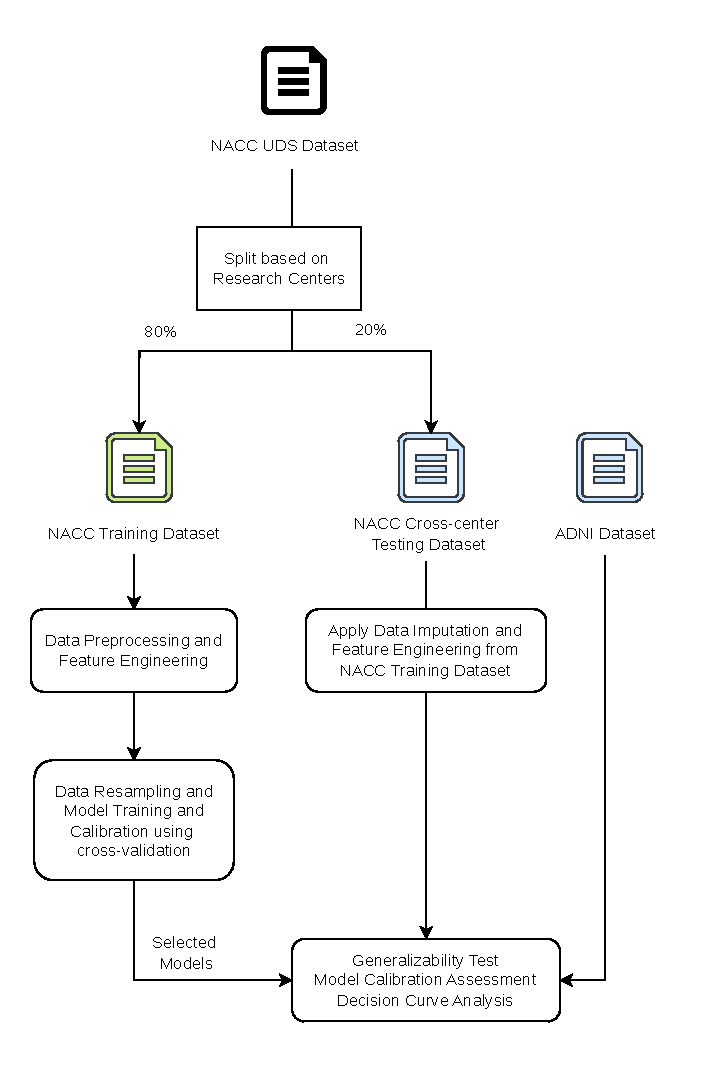
\includegraphics[width=0.65\textwidth]{figures/model-evaluation-diagram.pdf}
    \caption{Diagram of the model validation methodology and the dataset splitting strategy}
    \label{fig:model-validation}
\end{figure}

A deliberate selection of the model performance metrics is important for a reasonable evaluation of the classification models' performance. It can be observed that the datasets of all the binary classification tasks exhibit an imbalanced class distribution. Consequently, this study utilized a combination of performance metrics that account for class imbalance, such as sensitivity, specificity, G-mean, Area Under the Curve (\acrshort{AUC}), and F1-score. This is important to ensure a fair assessment of model performance in both majority and minority classes. In the medical field, it may also be more expensive to misclassify one class than the other. For example, classifying cognitively impaired cases as normal cases has a greater impact than classifying normal cases as cognitively impaired. Therefore, it is advisable to assess the true positive rate of the classification model. The distribution of the target classes in the NACC UDS and ADNI datasets for all classification tasks is provided in Figure~\ref{fig:nacc-data-stat} and Figure~\ref{fig:adni-data-stat} in the appendix, respectively.

In addition to evaluating the generalizability of the selected models, it is important to ensure that the models produce reliable probabilities of the targeted cognitive status or CI type (outcome). There is a possibility that even though a model with high classification accuracy could predict overly confident or conservative risk probabilities. In clinical application, an accurate estimate of how the outcome could possibly occur is required to make the right decision to manage any potential risk. Therefore, it is crucial that the predicted probability of the model approximates the actual likelihood of the outcome. For example, if a model predicts that there is an 80\% chance of cognitive impairment, about 80\% of subjects who get that prediction should have cognitive impairment.

Calibration was applied to the selected model using the beta calibration method to align their predicted probabilities with the actual risk of the outcome. The beta calibration works by fitting three parameters that learn how to transform the model's predicted probabilities to better match the actual likelihood of the risk. This method is more flexible than other approaches because it can correct both overconfidence and underestimation across different probability ranges. 

The beta calibration parameters were fitted using the model prediction in the stratified cross-validation out-of-fold (OOF). During the cross-validation, the model makes predictions on the validation fold (data it did not see during training). These OOF predictions were collected and used to train the beta calibration parameters. This ensures that the calibration is learned from unbiased model output. After that, the learned parameters were used to calibrate the model's predicted probabilities in external validation.

The effectiveness of the calibration was evaluated by comparing the uncalibrated and calibrated models in the NACC cross-center validation and the ADNI external validation using the following measures. These measures together provide a complete assessment of how well the model is calibrated.

\begin{itemize}
    \item \textbf{Calibration Curve:} A visual representation of the relationship between the model's predicted probabilities and the actual risk (diagonal line). A curve that follows the diagonal line indicates that the model is well calibrated. The calibration curve can help assess at which probability ranges the model is overconfident or underestimating the risk.
    \item \textbf{Brier score:} This is a widely used metric that evaluates the accuracy of the probabilities that the model predicts. It is calculated by taking the mean squared difference between the predicted probabilities and the actual outcomes. A Brier score below 0.20 means that the model prediction is accurate and calibrated.
    \item \textbf{Expected Calibration Error (\acrshort{ECE}):} This score measures the difference between the predicted probabilities and the observed frequencies. To calculate ECE, the model's predictions are divided into 10 bins. Then, the score is obtained by the weighted average of absolute differences between the mean predicted probability and the actual outcome frequency in each bin. In general, ECE values close to and below 0.05 indicate good calibration.
    \item \textbf{Intercept and Slope:} These values are obtained by a logistic regression model fitted to the calibration curve. An intercept below 0 indicates that the predicted probabilities are higher than the actual risk (the model is overestimating the risk), whereas an intercept above 0 indicates that the predicted probabilities are less than the actual risk (the model is underestimating the risk). The slope measures how well the model differentiates between different risk levels. A slope below 1 means the model is overconfident, pushing the predicted probabilities closer to 0 and 1, whereas a slope above 1 means the model is underconfident as it compresses probabilities around middle values (between 0.3 and 0.7). An intercept close to 0 and a slope close to 1 are considered measures of good calibration.
\end{itemize}
\vspace{2em}

After model calibration, the clinical utility of all classification and prediction models were assessed using Decision Curve Analysis (\acrshort{DCA}). This was done by calculating the model’s net benefit for different probability thresholds. DCA evaluates whether using these probabilities to guide clinical decisions provides additional value compared to alternative strategies like treat all and treat none.

\hl{This proposed validation method complies with the TRIPOD+AI guidelines} \cite{Collins2024TRIPOD+AI} \hl{through its focus on external validation, calibration, and clinical utility. Instead of relaying only on mathematical metrics, the predicted probabilities were assessed with calibration curves and clinical value was examined through decision curve analysis. Furthermore, the leave-multiple-center-out splitting follow recommendations from the literature} \cite{Christodoulou2019systematic}, \hl{which reported that validation procedures of machine learning models in clinical prediction are often biased and rarely calibrated.}

\section{Model Explainability}
The utility of a predictive model in a clinical setting goes beyond only prediction. It is necessary for the model prediction to be transparent, interpretable, and actionable. Since the objectives of this study are centered on the development of models that not only predict CI but also support personalized intervention plans, an XAI approach to model explainability is essential. 

The proposed XAI method in this study provides model explainability at multiple levels. The SHapley Additive exPlanations (\acrshort{SHAP}) \cite{Lundberg2017Unified} was used to provide global and individual explanations of the models’ predictions. This method computes Shapley values to quantify the contribution of each feature to a single model's prediction. For global explanation, the mean absolute Shapley values of each feature were calculated to determine the overall feature importance to the selected model. These values can be used to rank the features according to their overall importance to the model's prediction. This global explanation of the models is important to identify which risk factors (features) are the most strongly linked to cognitive impairment across the whole population. The feature importance was calculated on the ADNI external dataset, and it was compared to the feature importance on the NACC cross-center validation dataset using Spearman correlation. This comparison evaluates the stability of feature ranking across different datasets, which could demonstrate the generalizability of the model and the selected features.

In addition to the global explanation, the Shapley values were also used to explain the model prediction of individual instances. This local-level explanation clarifies why a specific instance got a particular prediction from the model. It helps answer questions like "What factors contributed to a case being classified as positive or negative?" which supports personalized risk communication and intervention. Shap waterfall plots were reported to demonstrate how correctly classified positive and negative cases with similar prediction probabilities have different feature contribution profiles. This assesses the capability of the selected model to capture specific risk patterns for different subjects. Although other local explanation methods like \acrshort{LIME} (Local Interpretable Model-agnostic Explanations) are used in the literature \cite{abbas2024Explainable, Vyas2022Identifying}, SHAP was utilized in this study because it is already used to compute the feature importance, and it has been widely used for global and individual explanation by other studies in CI and dementia research \cite{Beebe-Wang2021Efficient, Danso2021Developing, Yue2023Explainable}.

The XAI method in this study also leverages Diverse Counterfactual Explanations (\acrshort{DiCE}) \cite{Mothilal2019Explaining} to generate patient-specific counterfactual insights for risk management and intervention. For subjects predicted to have CIND or dementia, DiCE can propose a set of changes to their modifiable features that would be required to change the model's prediction to a desirable prediction (less severe cognitive status). A key advantage of DiCE is its ability to be configured to suggest changes only for features that can be modified (e.g., functional activities or scores from a Geriatric Depression Scale (\acrshort{GDS})), while keeping features such as gender and age static. For example, DiCE might suggest that a patient's cognitive status could improve from impaired to normal by managing the patient's GDS. This addresses this research objective to support the development of personalized risk management strategies. This counterfactual explanation was applied to all classification and prediction tasks in this study except the CI subtype classification task because the conversion from one CI subtype to another has no clinical value.

DiCE works by searching for different feature values that are similar to the original instance but result in different prediction outcomes. The goal is to minimize the distance between the original and counterfactual instances while ensuring that the desired outcome is obtained. In this research, the \acrshort{KD-Tree} (K-dimensional tree) search method was used to generate the counterfactual examples. This method builds a tree structure from the training data to search for nearest neighbors in the feature space that belong to the desired prediction class. The KD-Tree method was selected because it generates counterfactual examples that are based on real instances (training data) instead of generating synthetic examples that might not be feasible in practice. Additionally, it is computationally efficient for large datasets.

In this study, DiCE was configured to generate up to five counterfactual examples for each instance predicted as positive. The number of counterfactual examples generated per instance was analyzed to assess the ability of DiCE to find possible changes to improve cognitive status. The total number of features changed to generate counterfactual examples was also examined to evaluate the difficulty in applying the suggested interventions. DiCE also provides global importance scores for each feature based on how frequently it needs to be modified across all generated counterfactual examples. These scores were used to identify the most important features that could be utilized for risk interventions. Permitted values for certain features were defined, which were used by DiCE to generate realistic counterfactual examples. For example, the mass body index feature (NACCBMI) was configured with allowed values between 18.5 and 24.9, whereas the "never did" value in the FAQ features was set as disallowed.

In summary, the proposed XAI method was designed to provide both a global understanding of the selected models and patient-specific insights for CI risk prevention. It is achieved by the integration of SHAP for global feature importance and individual prediction explanations and DiCE for counterfactual insights. Consequently, the output of the models were transformed into a clinically meaningful and justifiable outcome. Therefore, it increases confidence in the model prediction and builds trust among clinicians and patients.

\hl{The results obtained from applying this methodology to the five classification and prediction tasks are presented and analyzed in the following chapter.}